% Options for packages loaded elsewhere
\PassOptionsToPackage{unicode}{hyperref}
\PassOptionsToPackage{hyphens}{url}
%
\documentclass[
  12pt,
  ignorenonframetext,
]{beamer}
\usepackage{pgfpages}
\setbeamertemplate{caption}[numbered]
\setbeamertemplate{caption label separator}{: }
\setbeamercolor{caption name}{fg=normal text.fg}
\beamertemplatenavigationsymbolsempty
% Prevent slide breaks in the middle of a paragraph
\widowpenalties 1 10000
\raggedbottom
\setbeamertemplate{part page}{
  \centering
  \begin{beamercolorbox}[sep=16pt,center]{part title}
    \usebeamerfont{part title}\insertpart\par
  \end{beamercolorbox}
}
\setbeamertemplate{section page}{
  \centering
  \begin{beamercolorbox}[sep=12pt,center]{part title}
    \usebeamerfont{section title}\insertsection\par
  \end{beamercolorbox}
}
\setbeamertemplate{subsection page}{
  \centering
  \begin{beamercolorbox}[sep=8pt,center]{part title}
    \usebeamerfont{subsection title}\insertsubsection\par
  \end{beamercolorbox}
}
\AtBeginPart{
  \frame{\partpage}
}
\AtBeginSection{
  \ifbibliography
  \else
    \frame{\sectionpage}
  \fi
}
\AtBeginSubsection{
  \frame{\subsectionpage}
}
\usepackage{amsmath,amssymb}
\usepackage{iftex}
\ifPDFTeX
  \usepackage[T1]{fontenc}
  \usepackage[utf8]{inputenc}
  \usepackage{textcomp} % provide euro and other symbols
\else % if luatex or xetex
  \usepackage{unicode-math} % this also loads fontspec
  \defaultfontfeatures{Scale=MatchLowercase}
  \defaultfontfeatures[\rmfamily]{Ligatures=TeX,Scale=1}
\fi
\usepackage{lmodern}
\ifPDFTeX\else
  % xetex/luatex font selection
\fi
% Use upquote if available, for straight quotes in verbatim environments
\IfFileExists{upquote.sty}{\usepackage{upquote}}{}
\IfFileExists{microtype.sty}{% use microtype if available
  \usepackage[]{microtype}
  \UseMicrotypeSet[protrusion]{basicmath} % disable protrusion for tt fonts
}{}
\makeatletter
\@ifundefined{KOMAClassName}{% if non-KOMA class
  \IfFileExists{parskip.sty}{%
    \usepackage{parskip}
  }{% else
    \setlength{\parindent}{0pt}
    \setlength{\parskip}{6pt plus 2pt minus 1pt}}
}{% if KOMA class
  \KOMAoptions{parskip=half}}
\makeatother
\usepackage{xcolor}
\newif\ifbibliography
\usepackage{graphicx}
\makeatletter
\def\maxwidth{\ifdim\Gin@nat@width>\linewidth\linewidth\else\Gin@nat@width\fi}
\def\maxheight{\ifdim\Gin@nat@height>\textheight\textheight\else\Gin@nat@height\fi}
\makeatother
% Scale images if necessary, so that they will not overflow the page
% margins by default, and it is still possible to overwrite the defaults
% using explicit options in \includegraphics[width, height, ...]{}
\setkeys{Gin}{width=\maxwidth,height=\maxheight,keepaspectratio}
% Set default figure placement to htbp
\makeatletter
\def\fps@figure{htbp}
\makeatother
\setlength{\emergencystretch}{3em} % prevent overfull lines
\providecommand{\tightlist}{%
  \setlength{\itemsep}{0pt}\setlength{\parskip}{0pt}}
\setcounter{secnumdepth}{-\maxdimen} % remove section numbering
\usetheme{boxes}
%\usetheme{madrid} 
%\usetheme{metropolis} 
%\usetheme{Boadilla} 

%   \setbeameroption{show notes}  %the default is not to show notes

\usepackage{amsmath}
\setbeamertemplate{itemize items}[ball]
\setbeamertemplate{itemize subitem}[dash]
%\setbeamertemplate{frametitle}[default][center]
\setbeamertemplate{frametitle}[default][left]

%\setbeamertemplate{note page}[plain]
%\setbeamertemplate{note page}{\pagecolor{yellow!5}\insertnote}
\setbeamertemplate{note page}{\pagecolor{gray!15}\insertnote}

\usepackage[abs]{overpic}
\usepackage{wrapfig}
%\usepackage[table]{xcolor}
\usepackage{booktabs} %\toprule (and \midrule or \bottomrule) are defined in the booktabs package. 
%\usepackage{tabu}
\usepackage{longtable}
\usepackage{array}
\usepackage{multirow}
\usepackage{float}
\usepackage[most]{tcolorbox} %doesn't clash with the below
\usepackage{colortbl} 
\usepackage{pdflscape}
\usepackage{tabu}
\usepackage{threeparttable}
\usepackage{threeparttablex}
\usepackage[normalem]{ulem}
\usepackage{makecell}

% \usepackage{xcolor} %clashes with  \usepackage{colortbl}

\AtBeginNote{\hspace*{-5pt}\addtolength\leftmargini{-10pt}}
\AtEndNote{\addtolength\leftmargini{5pt}}

%\beamertemplatenavigationsymbolsempty
%\setbeamerfont{page number in head/foot}{size=\large}
\setbeamertemplate{footline}[frame number]                                       %page number

% defining a color
\definecolor{mossgreen}{rgb}{0.68, 0.87, 0.68}
\usepackage{mdframed}
\usepackage{framed}
\usepackage{scalerel,stackengine}

\usepackage{blindtext} %This package generates automatic text
\usepackage{epigraph}
\setlength\epigraphwidth{10cm}
\setlength\epigraphrule{0pt}
\makeatletter
\patchcmd{\epigraph}{\@epitext{#1}}{\itshape\@epitext{#1}}{}{}
\makeatother
\ifLuaTeX
  \usepackage{selnolig}  % disable illegal ligatures
\fi
\IfFileExists{bookmark.sty}{\usepackage{bookmark}}{\usepackage{hyperref}}
\IfFileExists{xurl.sty}{\usepackage{xurl}}{} % add URL line breaks if available
\urlstyle{same}
\hypersetup{
  pdftitle={Thinking Like an Economist},
  pdfauthor={Abel Embaye},
  hidelinks,
  pdfcreator={LaTeX via pandoc}}

\title{Thinking Like an Economist}
\author{Abel Embaye}
\date{September 08, 2025}
\institute{Department of Economics\\
\strut \\
UofA\\}

\begin{document}
\frame{\titlepage}

\begin{frame}{Chapter Outline}
\protect\hypertarget{chapter-outline}{}
Chapter Outline

13.1 Aggregate Demand + 13.2 Aggregate Supply + 13.3 Macroeconomic
Equilibrium in the Long Run and the Short Run + 13.4 A Dynamic Aggregate
Demand and Aggregate Supply Model + Appendix Macroeconomic Schools of
Thought
\end{frame}

\begin{frame}{A M C and D. R. Horton Switch Places}
\protect\hypertarget{a-m-c-and-d.-r.-horton-switch-places}{}
A M C and D. R. Horton Switch Places

If the U.S. economy was about to enter a recession, would you prefer to
work for movie chain A M C or home builder D. R. Horton? + In normal
recessions, A M C would win out. However, in the Covid-19 recession
spending on services declined by 3 percent while residential
construction increased 21 percent, spurred on by record low interest
rates and stimulus checks. + A M C was hit hard by social distancing
rules and forced closures while D. R. Horton's revenues increased.

\includegraphics[width=\textwidth,height=0.99\textheight]{imgs3/img_slide03a.png}
\end{frame}

\begin{frame}{13.1 Aggregate Demand}
\protect\hypertarget{aggregate-demand}{}
13.1 Aggregate Demand

Identify the determinants of aggregate demand and distinguish between a
movement along the aggregate demand curve and a shift of the curve.

Real G D P has four components: + Consumption (C) + Investment (I) +
Government purchases (G) + Net exports (N X)

Adding these gives real G D P:

Government purchases are generally determined by the decisions of
policymakers and are independent of changes in the price level. +
However, consumption, investment, and net exports are affected by
changes in the price level. We will examine each in turn.
\end{frame}

\begin{frame}{Aggregate Demand and Aggregate Supply Model}
\protect\hypertarget{aggregate-demand-and-aggregate-supply-model}{}
Aggregate Demand and Aggregate Supply Model

We have now modeled long-run economic growth and also how real G D P is
determined in the short run. + New goal: extend the model of the economy
in the short run in order to explain why the following fluctuate: + Real
G D P + Employment + The price level

New model: Aggregate demand and aggregate supply model, a model that
explains short-run fluctuations in real G D P and the price level.
\end{frame}

\begin{frame}{Figure 13.1 Aggregate Demand and Aggregate Supply (1 of
3)}
\protect\hypertarget{figure-13.1-aggregate-demand-and-aggregate-supply-1-of-3}{}
Figure 13.1 Aggregate Demand and Aggregate Supply (1 of 3)

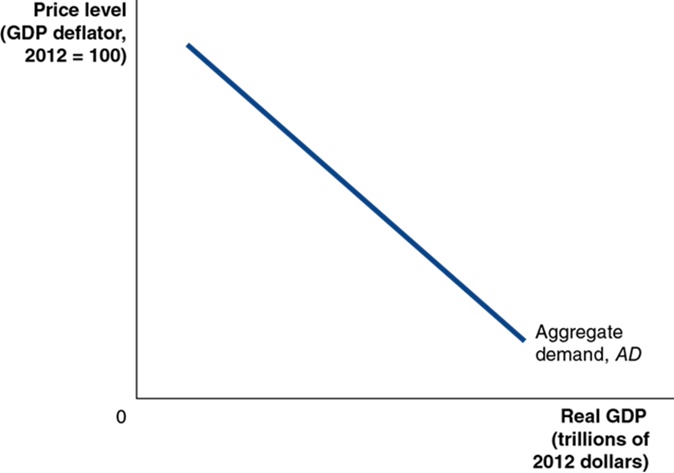
\includegraphics[width=\textwidth,height=0.99\textheight]{imgs3/img_slide06a.png}

In the short run, real G D P and the price level are determined by the
intersection of the aggregate demand curve. . . + Aggregate demand (A D)
curve: A curve that shows the relationship between the price level and
the quantity of real G D P demanded by households, firms, and the
government (both inside and outside of the country).
\end{frame}

\begin{frame}{Figure 13.1 Aggregate Demand and Aggregate Supply (2 of
3)}
\protect\hypertarget{figure-13.1-aggregate-demand-and-aggregate-supply-2-of-3}{}
Figure 13.1 Aggregate Demand and Aggregate Supply (2 of 3)

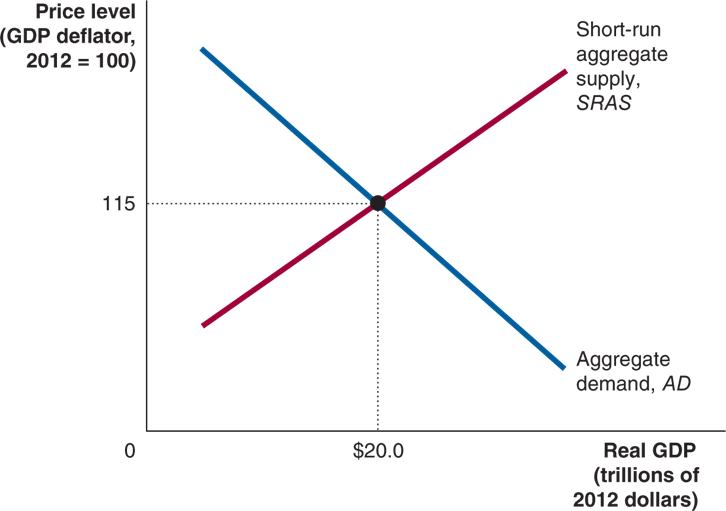
\includegraphics[width=\textwidth,height=0.99\textheight]{imgs3/img_slide07a.png}

\ldots and the short-run aggregate supply curve. + Short-run aggregate
supply (S R A S) curve: A curve that shows the relationship in the short
run between the price level and the quantity of real G D P supplied by
firms.
\end{frame}

\begin{frame}{The Wealth Effect: How a Change in the Price Level Affects
Consumption}
\protect\hypertarget{the-wealth-effect-how-a-change-in-the-price-level-affects-consumption}{}
The Wealth Effect: How a Change in the Price Level Affects Consumption

Household consumption is most strongly determined by income, but it is
also affected by wealth. + Some household wealth is held in nominal
assets, so as price levels rise, the real value of household wealth
declines. This results in less consumption. + Implication: higher price
level leads to lower consumption.
\end{frame}

\begin{frame}{The Interest-Rate Effect: How a Change in the Price Level
Affects Investment}
\protect\hypertarget{the-interest-rate-effect-how-a-change-in-the-price-level-affects-investment}{}
The Interest-Rate Effect: How a Change in the Price Level Affects
Investment

When prices rise, households and firms need more money to finance buying
and selling. + So, households and firms borrow and withdraw funds from
banks and sell financial assets such as bonds in order to have more
funds available. + This increase in demand for money causes the
``price'' of holding money (the interest rate) to rise, discouraging
firm investment. + Implication: higher price level leads to lower
investment.
\end{frame}

\begin{frame}{The International-Trade Effect: How a Change in the Price
Level Affects Net Exports}
\protect\hypertarget{the-international-trade-effect-how-a-change-in-the-price-level-affects-net-exports}{}
The International-Trade Effect: How a Change in the Price Level Affects
Net Exports

When U.S. price levels rise, U.S. exports become more expensive and
imports become relatively cheaper. + Fewer exports and more imports mean
net exports falls. + Implication: higher price level leads to lower net
exports.
\end{frame}

\begin{frame}{Figure 13.1 Aggregate Demand and Aggregate Supply (3 of
3)}
\protect\hypertarget{figure-13.1-aggregate-demand-and-aggregate-supply-3-of-3}{}
Figure 13.1 Aggregate Demand and Aggregate Supply (3 of 3)

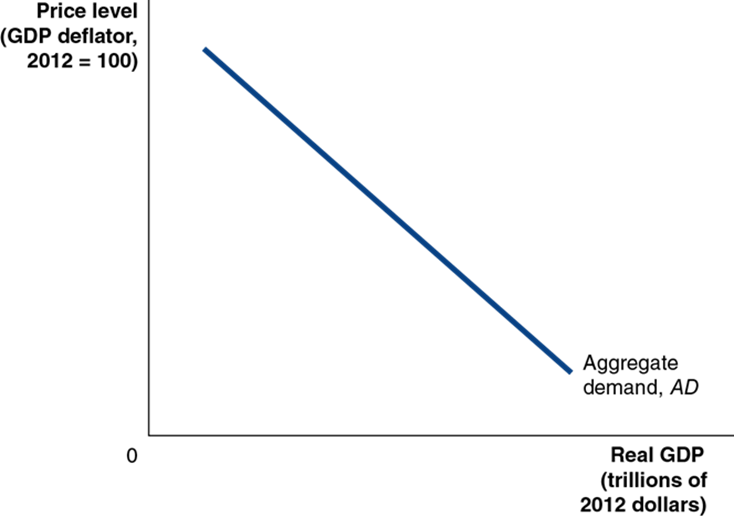
\includegraphics[width=\textwidth,height=0.99\textheight]{imgs3/img_slide11a.png}

Each of the three effects show higher price levels leading to lower
values of components of real G D P. + This establishes that the
aggregate demand curve slopes downward.
\end{frame}

\begin{frame}{Shifts of the Aggregate Demand Curve versus Movements
along It}
\protect\hypertarget{shifts-of-the-aggregate-demand-curve-versus-movements-along-it}{}
Shifts of the Aggregate Demand Curve versus Movements along It

The aggregate demand curve shows the relationship between the price
level and real G D P demanded, holding everything else constant. + A
movement along the A D curve will occur when the price level changes,
and the change in prices is not caused by a component of real G D P
changing. + A shift of the A D curve will occur when some component of
real G D P changes; for example, a change in government purchases.
\end{frame}

\begin{frame}{Table 13.1 Variables That Shift the Aggregate Demand Curve
(1 of 4)}
\protect\hypertarget{table-13.1-variables-that-shift-the-aggregate-demand-curve-1-of-4}{}
Table 13.1 Variables That Shift the Aggregate Demand Curve (1 of 4)

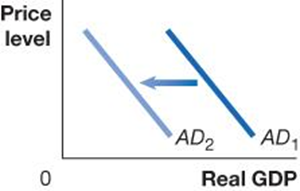
\includegraphics[width=\textwidth,height=0.99\textheight]{imgs3/img_slide13a.png}

A government policy change could shift aggregate demand. There are two
categories of government policies here: + Monetary policy: The actions
the Federal Reserve takes to manage the money supply and interest rates
to pursue macroeconomic policy objectives.

If the Federal Reserve causes interest rates to rise, investment
spending will fall; if it causes interest rates to fall, investment
spending will rise.
\end{frame}

\begin{frame}{Table 13.1 Variables That Shift the Aggregate Demand Curve
(2 of 4)}
\protect\hypertarget{table-13.1-variables-that-shift-the-aggregate-demand-curve-2-of-4}{}
Table 13.1 Variables That Shift the Aggregate Demand Curve (2 of 4)

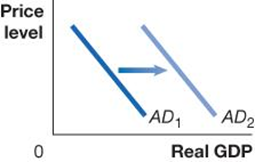
\includegraphics[width=\textwidth,height=0.99\textheight]{imgs3/img_slide14a.png}

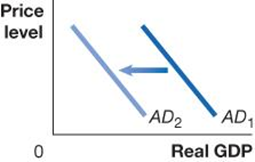
\includegraphics[width=\textwidth,height=0.99\textheight]{imgs3/img_slide14b.png}

Fiscal policy: Changes in federal taxes and purchases that are intended
to achieve macroeconomic policy objectives.

Increasing or decreasing personal income taxes affects disposable income
and hence consumption. The government can also alter its level of
government purchases. It could also alter business taxes, affecting the
level of investment spending.
\end{frame}

\begin{frame}{Table 13.1 Variables That Shift the Aggregate Demand Curve
(3 of 4)}
\protect\hypertarget{table-13.1-variables-that-shift-the-aggregate-demand-curve-3-of-4}{}
Table 13.1 Variables That Shift the Aggregate Demand Curve (3 of 4)

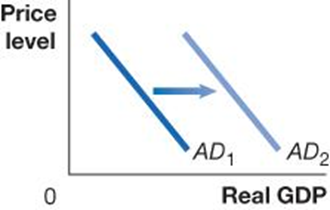
\includegraphics[width=\textwidth,height=0.99\textheight]{imgs3/img_slide15a.png}

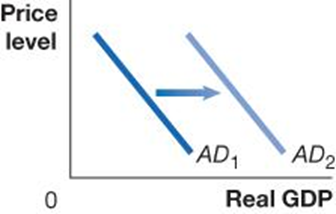
\includegraphics[width=\textwidth,height=0.99\textheight]{imgs3/img_slide15b.png}

Households or firms could become more optimistic about the future,
increasing consumption or investment, respectively. + Of course, the
opposite could also occur.
\end{frame}

\begin{frame}{Table 13.1 Variables That Shift the Aggregate Demand Curve
(4 of 4)}
\protect\hypertarget{table-13.1-variables-that-shift-the-aggregate-demand-curve-4-of-4}{}
Table 13.1 Variables That Shift the Aggregate Demand Curve (4 of 4)

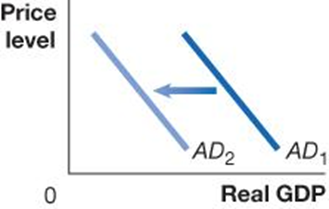
\includegraphics[width=\textwidth,height=0.99\textheight]{imgs3/img_slide16a.png}

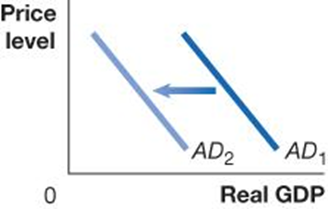
\includegraphics[width=\textwidth,height=0.99\textheight]{imgs3/img_slide16b.png}

If foreign incomes rise more slowly than ours, their imports of our
goods fall; if ours rise more slowly, our imports fall. + If our
exchange rate (the value of the \$U S) rises, our exports become more
expensive, so foreigners buy less of them (and we buy more imports,
also).
\end{frame}

\begin{frame}{Apply the Concept: Which Components of Aggregate Demand
Changed the Most during the 2020 Recession? (1 of 3)}
\protect\hypertarget{apply-the-concept-which-components-of-aggregate-demand-changed-the-most-during-the-2020-recession-1-of-3}{}
Apply the Concept: Which Components of Aggregate Demand Changed the Most
during the 2020 Recession? (1 of 3)

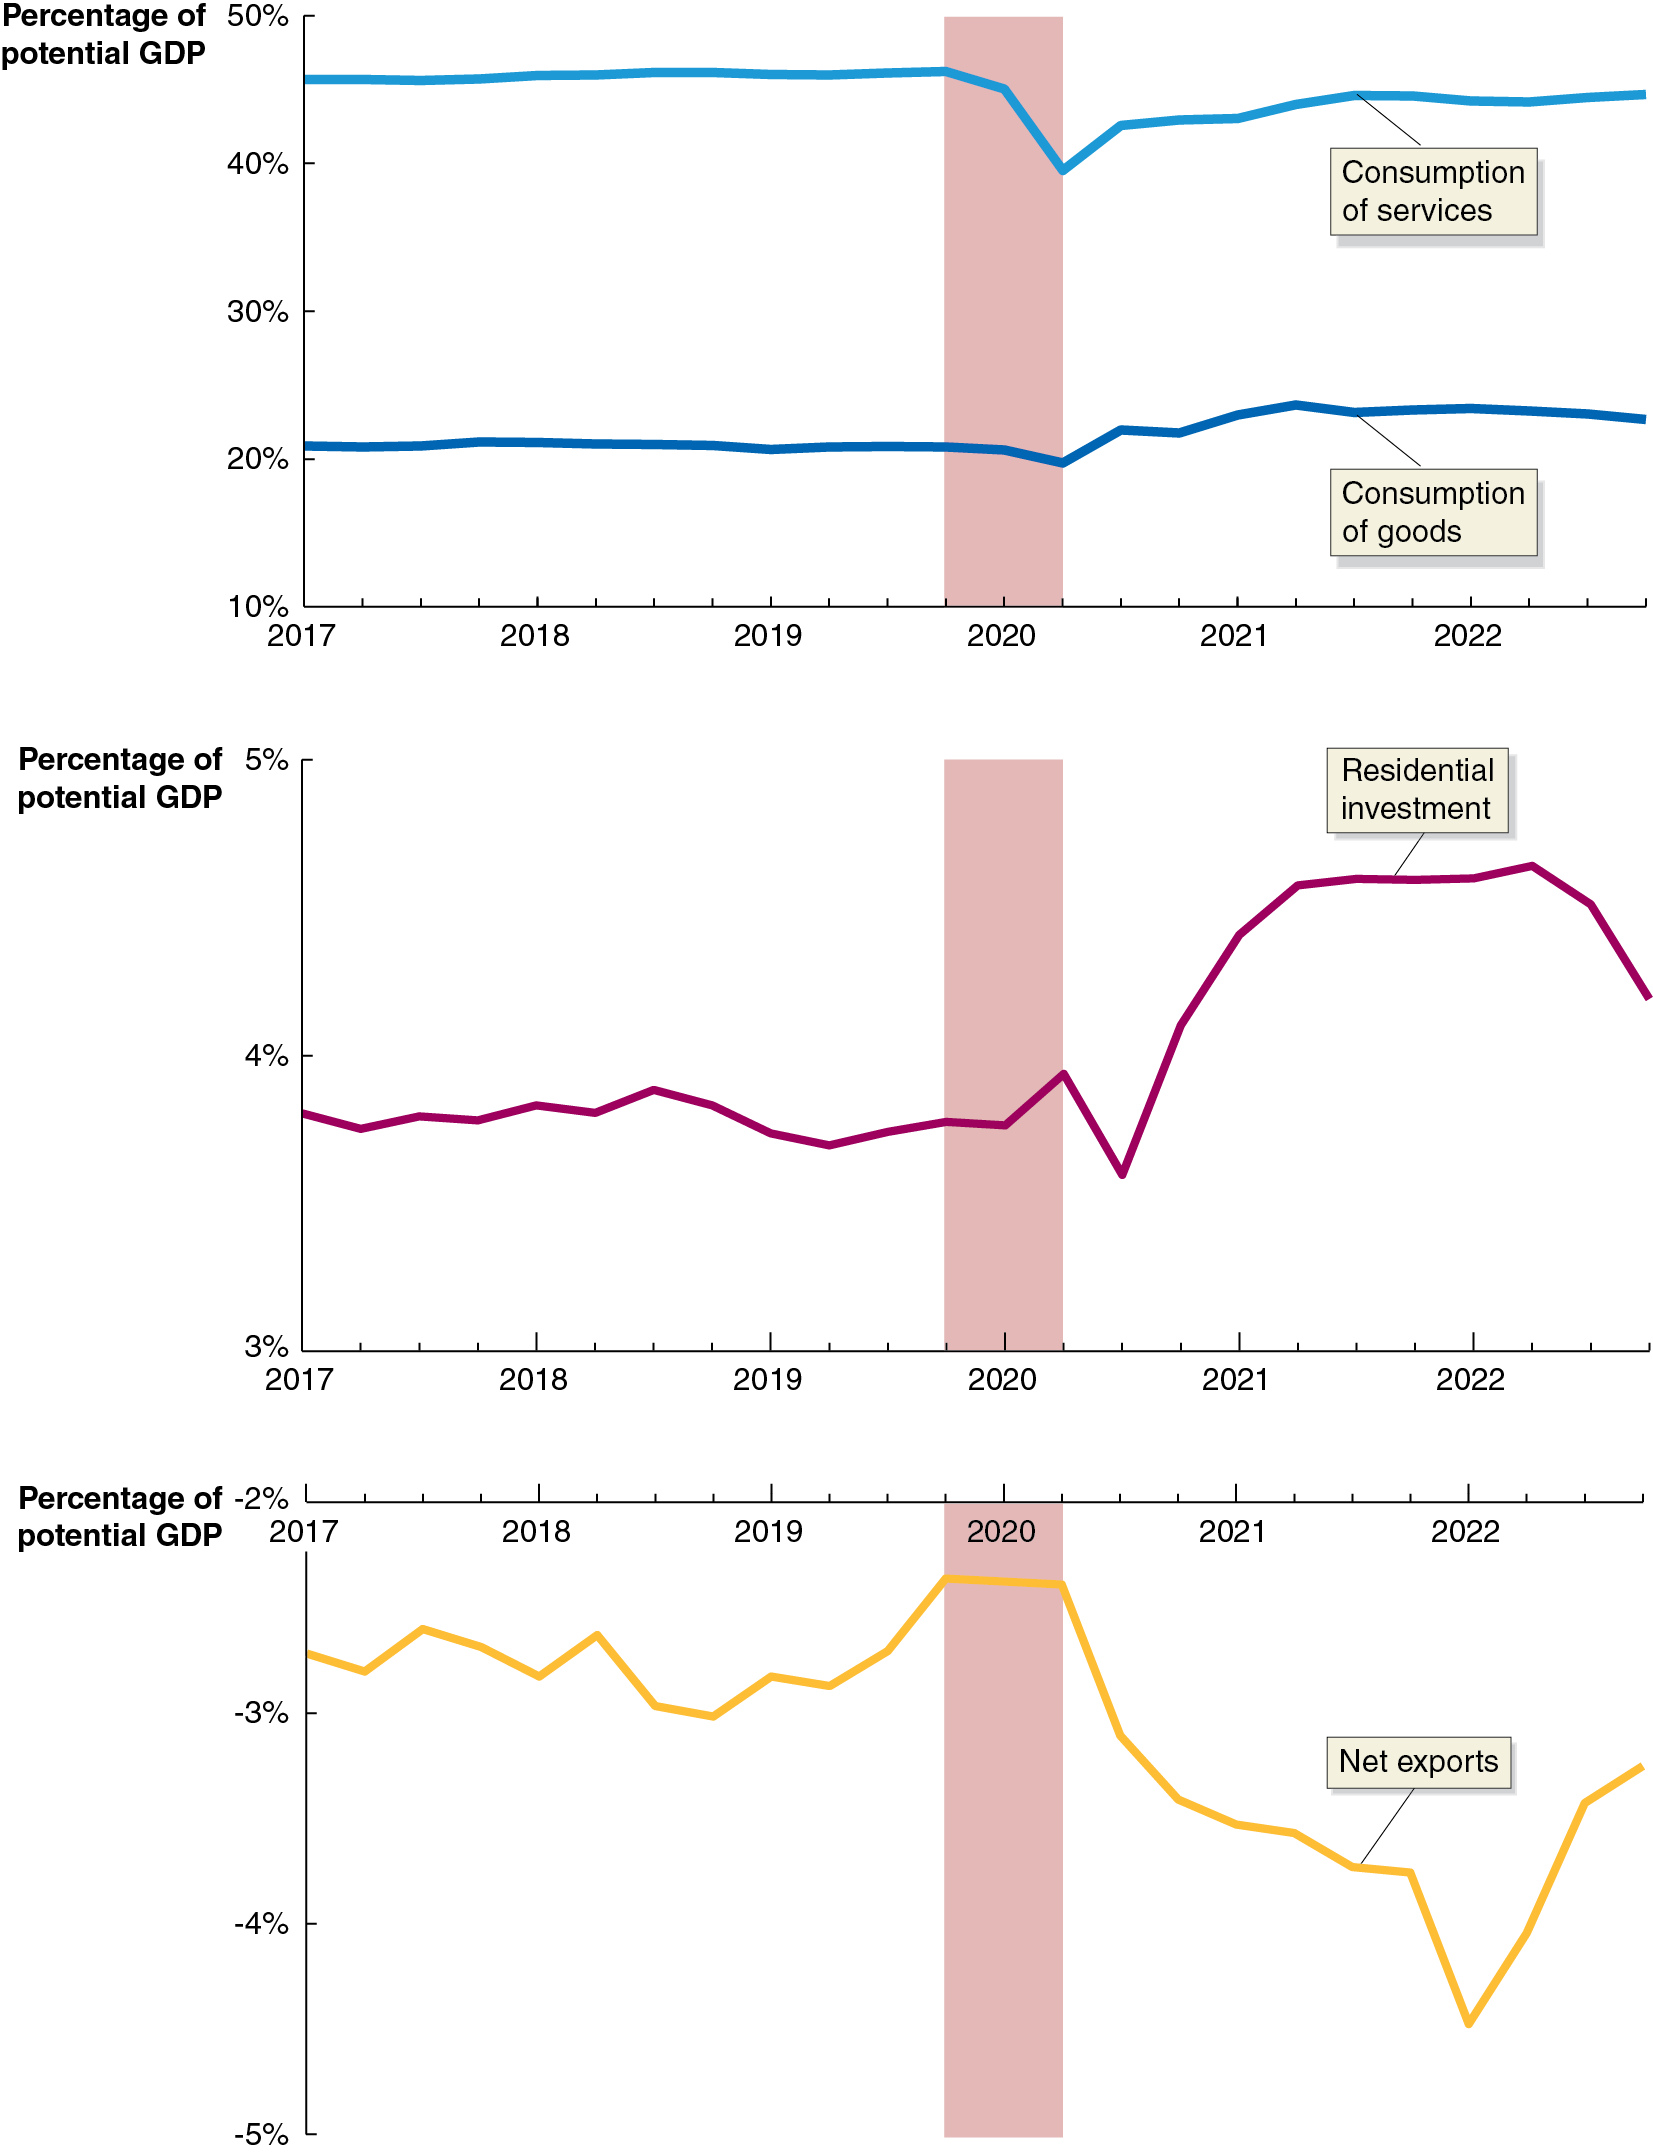
\includegraphics[width=\textwidth,height=0.99\textheight]{imgs3/img_slide17a.png}

We can understand the 2020 recession better by examining what happened
to the components of real G D P. + Consumption spending fell, relative
to potential G D P, during the recession. + Spending on services fell
sharply while spending on goods fell slightly before increasing and then
stabilizing.
\end{frame}

\begin{frame}{Apply the Concept: Which Components of Aggregate Demand
Changed the Most during the 2020 Recession? (2 of 3)}
\protect\hypertarget{apply-the-concept-which-components-of-aggregate-demand-changed-the-most-during-the-2020-recession-2-of-3}{}
Apply the Concept: Which Components of Aggregate Demand Changed the Most
during the 2020 Recession? (2 of 3)

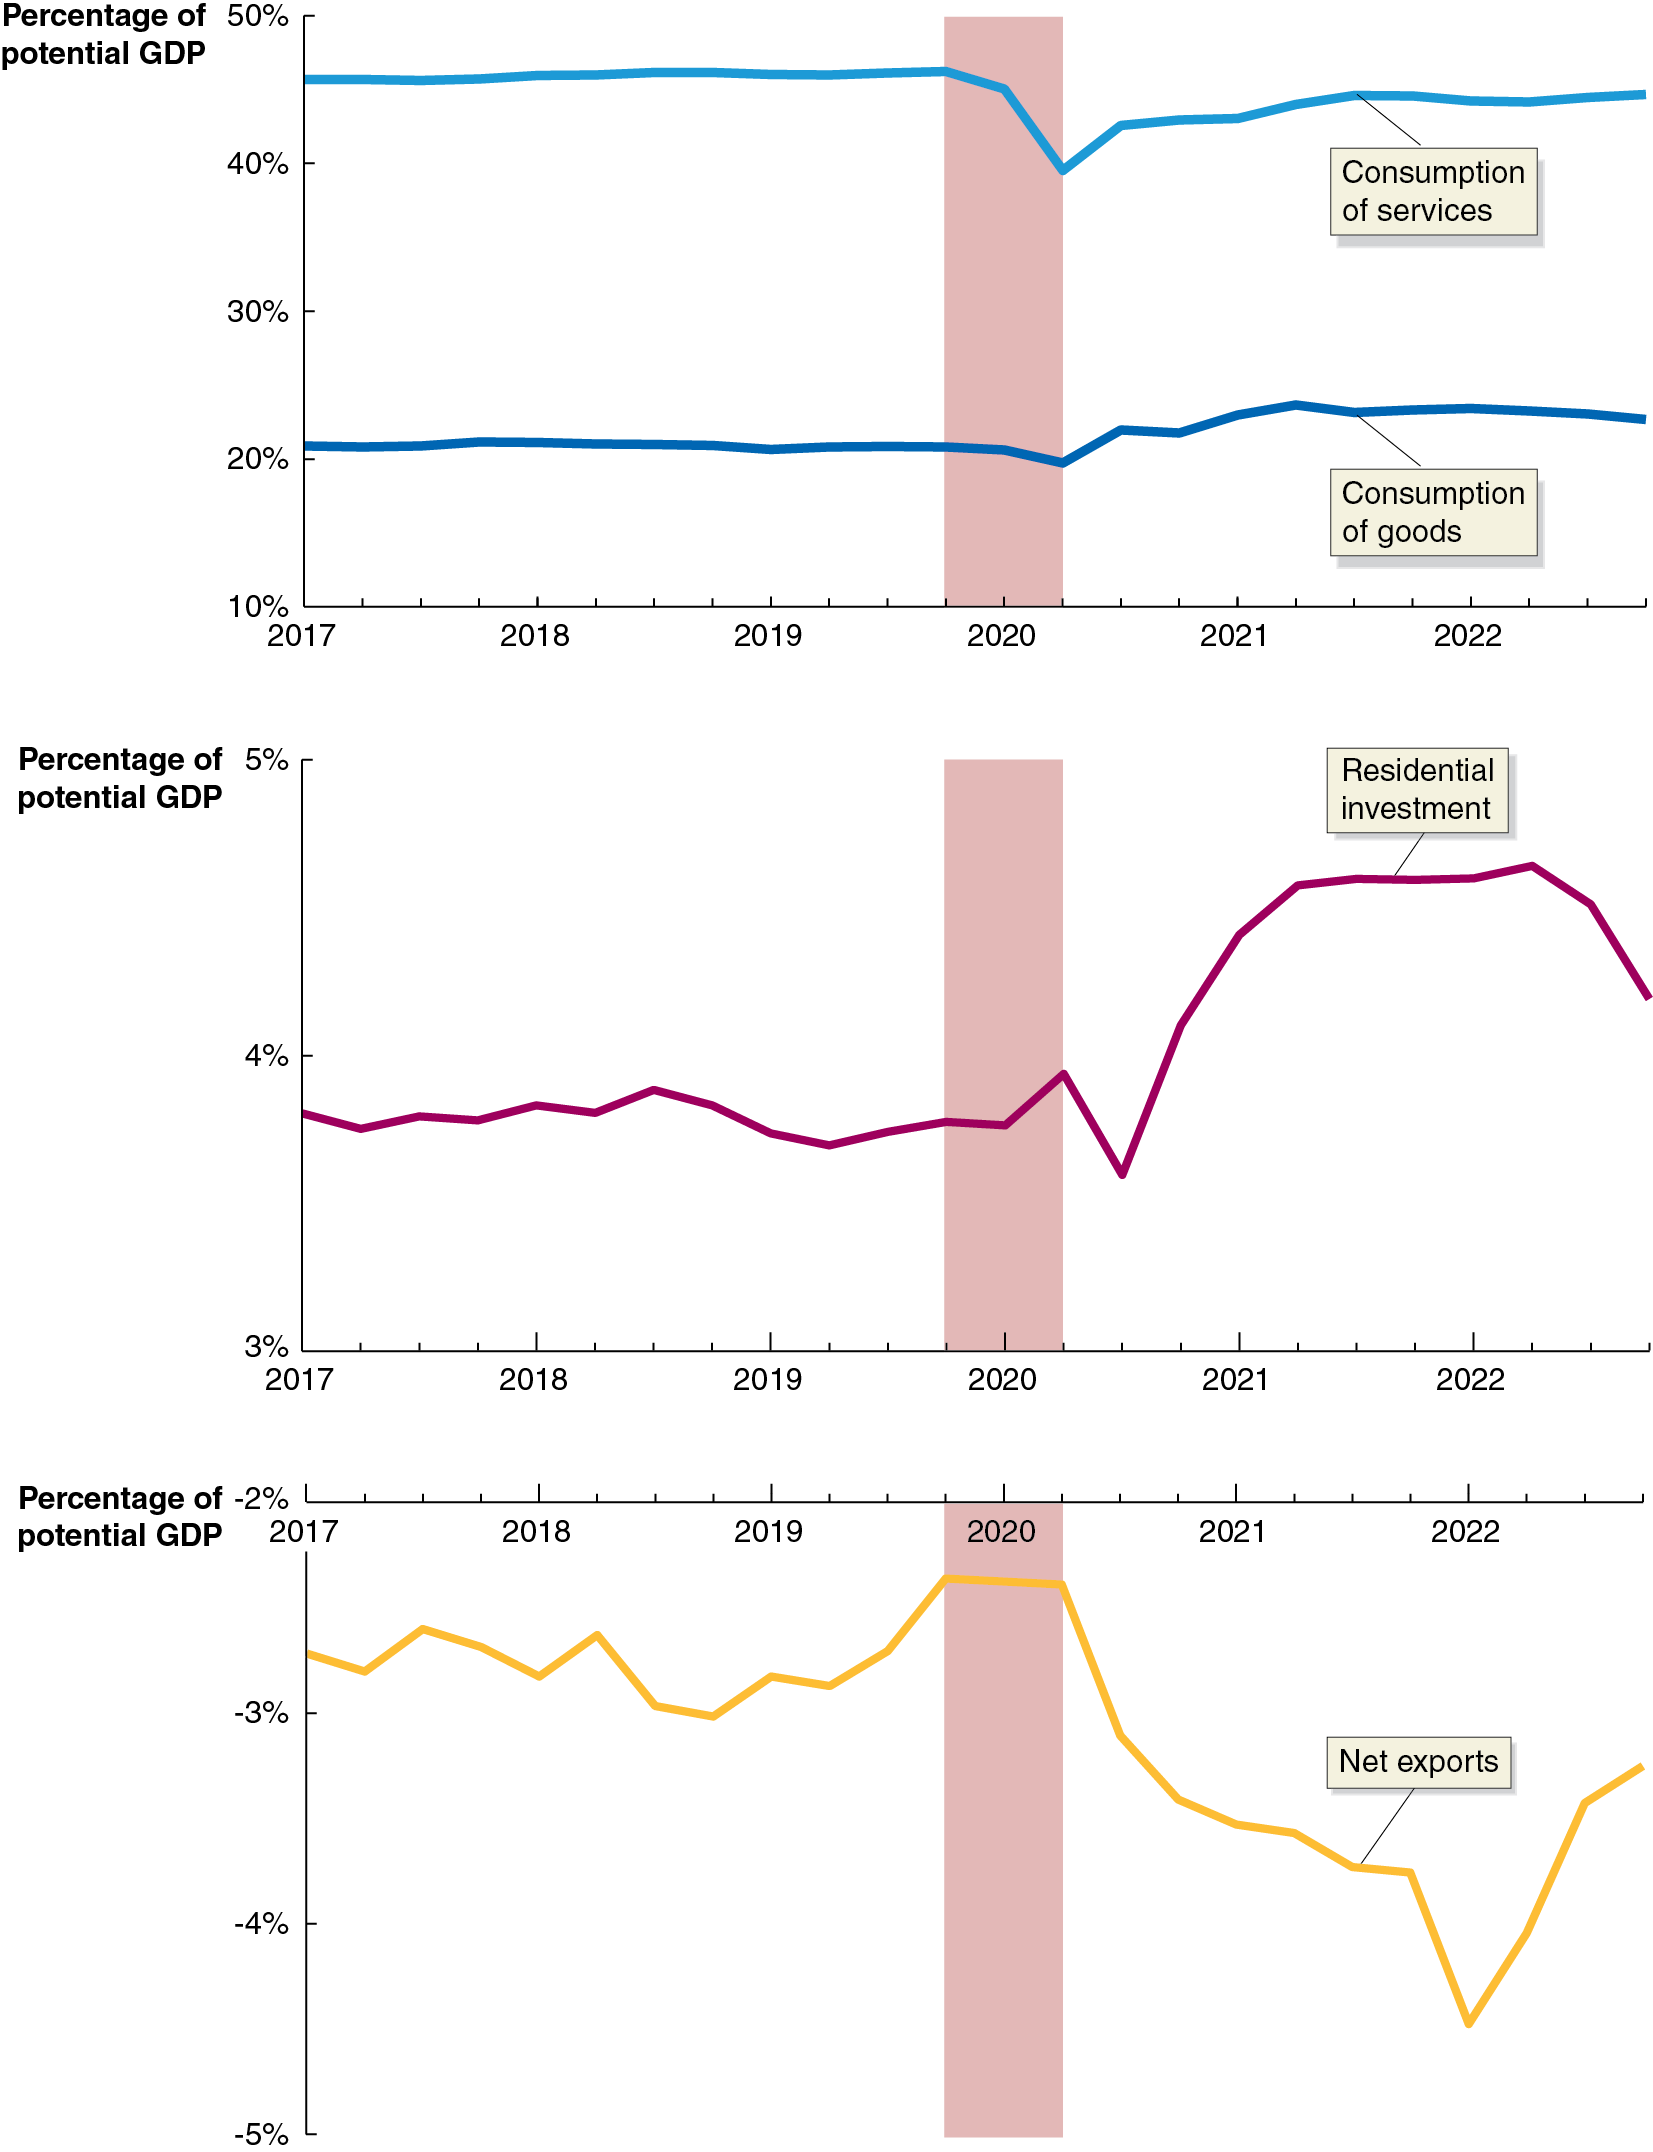
\includegraphics[width=\textwidth,height=0.99\textheight]{imgs3/img_slide18a.png}

Residential investment had been stable before the recession and
initially fell during the first part of the 2020 recession. + However,
the housing market pulled residential investment up due to continued low
interest rates and consumers with excess stimulus cash. + Residential
investment increased sharply in the latter part of the 2020 recession,
and stayed high for the following couple of years.
\end{frame}

\begin{frame}{Apply the Concept: Which Components of Aggregate Demand
Changed the Most during the 2020 Recession? (3 of 3)}
\protect\hypertarget{apply-the-concept-which-components-of-aggregate-demand-changed-the-most-during-the-2020-recession-3-of-3}{}
Apply the Concept: Which Components of Aggregate Demand Changed the Most
during the 2020 Recession? (3 of 3)

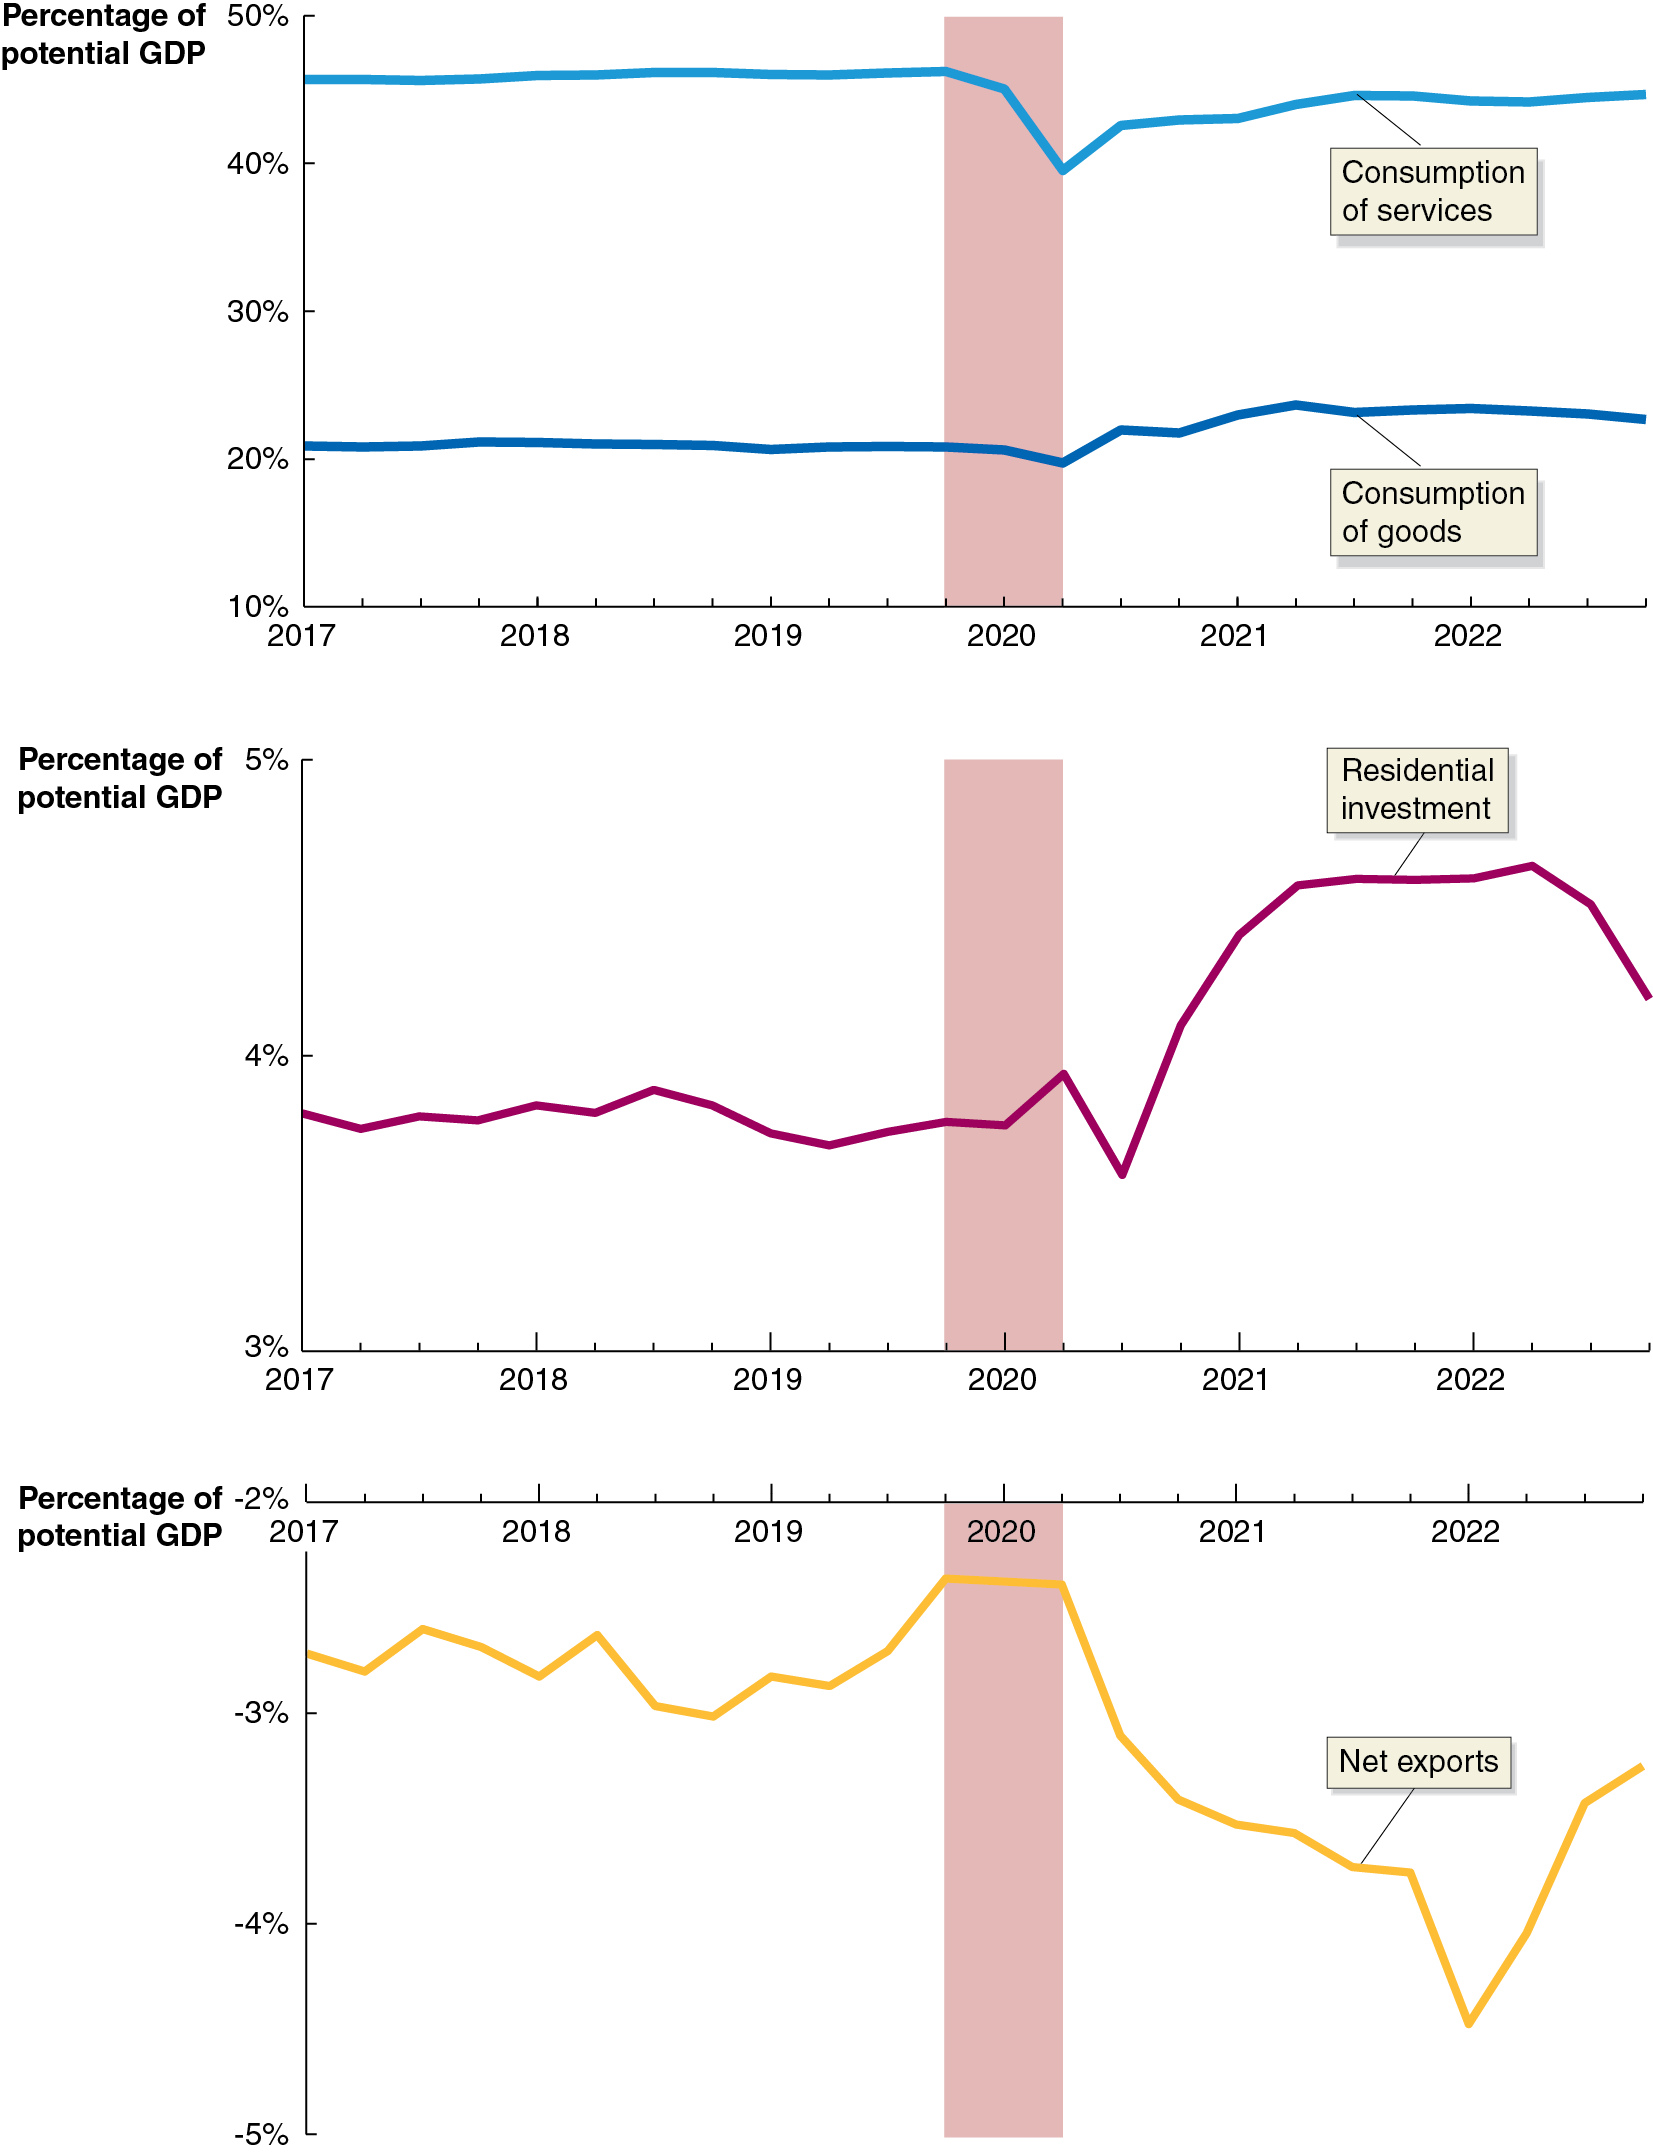
\includegraphics[width=\textwidth,height=0.99\textheight]{imgs3/img_slide19a.png}

Net exports decreased during and after the recession. (Because net
exports was negative throughout this period, it decreased by becoming a
larger negative number.) + This was in part due to a sharp increase in
the value of the \$U S. + U .S. G D P also fell less than our trading
partners, pushing net exports lower.
\end{frame}

\begin{frame}{13.2 Aggregate Supply}
\protect\hypertarget{aggregate-supply}{}
13.2 Aggregate Supply

Identify the determinants of aggregate supply and distinguish between a
movement along the short-run aggregate supply curve and a shift of the
curve.

Aggregate supply refers to the quantity of goods and services that firms
are willing and able to supply. + The relationship between this quantity
and the price level is different in the long and short run. + So, we
will develop both a short-run and long-run aggregate supply curve.

Long-run aggregate supply (L R A S) curve: A curve that shows the
relationship in the long run between the price level and the quantity of
real G D P supplied.
\end{frame}

\begin{frame}{Figure 13.2 The Long-Run Aggregate Supply Curve}
\protect\hypertarget{figure-13.2-the-long-run-aggregate-supply-curve}{}
Figure 13.2 The Long-Run Aggregate Supply Curve

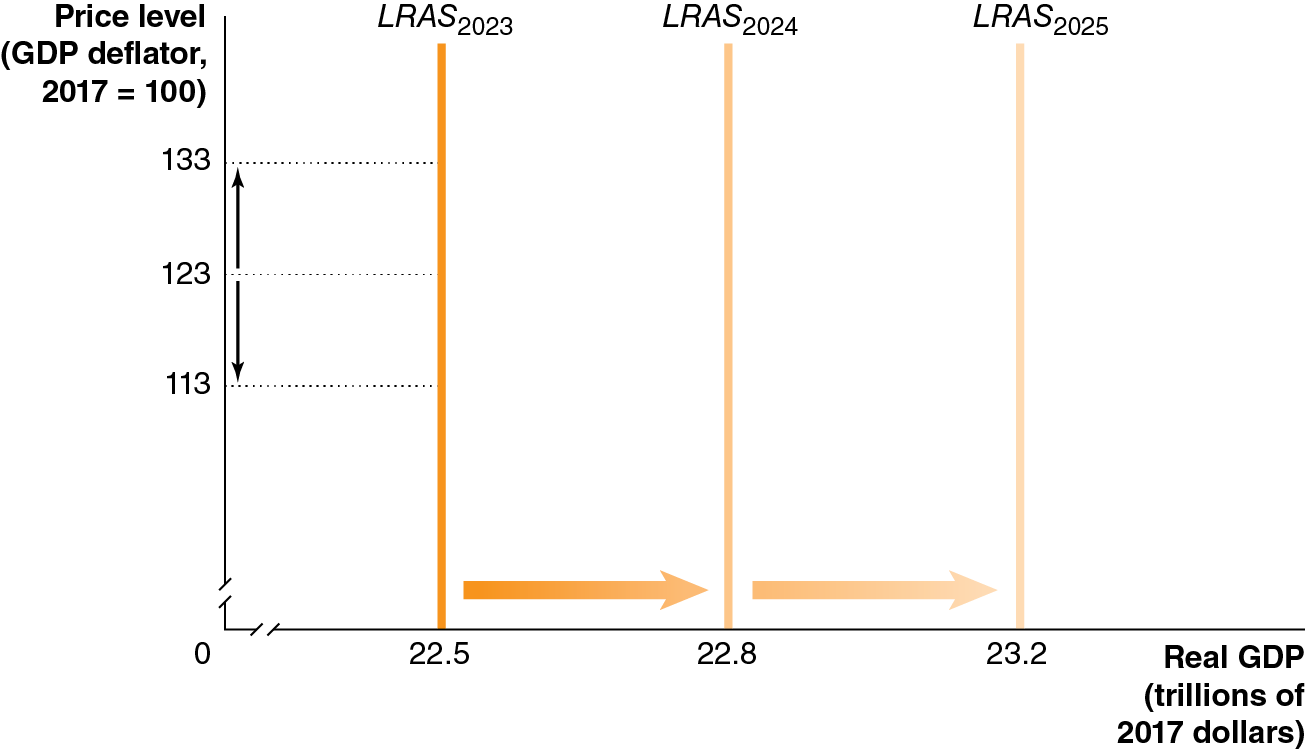
\includegraphics[width=\textwidth,height=0.99\textheight]{imgs3/img_slide21a.png}

In the long run, the level of real G D P is determined by the number of
workers, the level of technology, and the capital stock (factories,
machinery, etc.). + None of these elements is affected by the price
level, so L R A S does not depend on the price level; it is a vertical
line. + L R AS occurs at the level of potential or full-employment G D
P, which advances each year.
\end{frame}

\begin{frame}{The Short-Run Aggregate Supply Curve}
\protect\hypertarget{the-short-run-aggregate-supply-curve}{}
The Short-Run Aggregate Supply Curve

While the L R A S is vertical, the S R A S is upward sloping. Why? + As
prices of final goods and services rise, prices of inputs---such as the
wages of workers or the price of natural resources---rise more slowly. +
A secondary reason is that some firms are slow to adjust their prices
when the price level rises or falls.

Economists tend to believe that some firms and workers fail to
accurately predict changes in the price level. This gives us three
potential explanations for why the S R A S curve is upward sloping: +
Contracts make some wages and prices ``sticky''. + Firms are often slow
to adjust wages. + Menu costs make some prices sticky.
\end{frame}

\begin{frame}{Why Is the S R A S Curve Upward Sloping?}
\protect\hypertarget{why-is-the-s-r-a-s-curve-upward-sloping}{}
Why Is the S R A S Curve Upward Sloping?

Contracts make some wages and prices ``sticky''

Prices and wages are said to be ``sticky'' when they do not respond
quickly to changes in demand or supply. + Some firms and workers fail to
predict price level changes, and so do not correctly build them into
long-term contracts.

Firms are often slow to adjust wages

Salary reviews typically only happen annually. + Also, firms dislike
cutting wages---it's bad for morale.

Menu costs make some prices sticky

Firms have menu costs: The costs to firms of changing prices. + A small
``optimal'' change in price may not be worth the hassle for a firm to
perform.
\end{frame}

\begin{frame}{Apply the Concept: How Sticky Are Wages?}
\protect\hypertarget{apply-the-concept-how-sticky-are-wages}{}
Apply the Concept: How Sticky Are Wages?

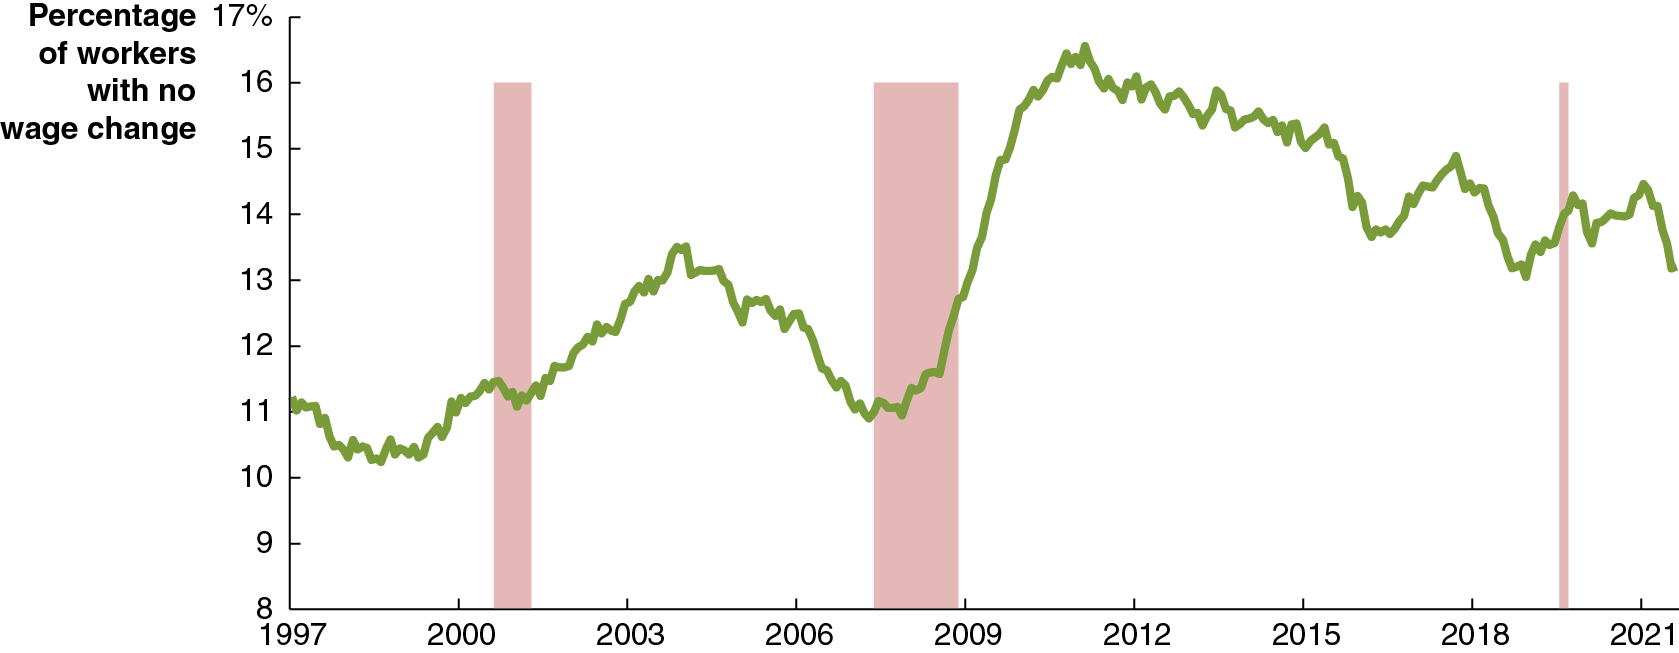
\includegraphics[width=\textwidth,height=0.99\textheight]{imgs3/img_slide24a.png}

It is unclear how sticky wages are. There is good evidence that wages
are at least sticky downward. + Instead of cutting (nominal) wages,
firms tend to fire current workers, freeze pay, and offer lower salaries
to new workers. This ``gets misery out of the door.''

The graph shows the percentage of workers with no wage change in a given
year.
\end{frame}

\begin{frame}{Shifts of the S R A S Curve versus Movements Along It}
\protect\hypertarget{shifts-of-the-s-r-a-s-curve-versus-movements-along-it}{}
Shifts of the S R A S Curve versus Movements Along It

The short-run aggregate supply curve (S R A S) describes the
relationship between the price level and the quantity of goods and
services firms are willing to supply, holding constant all other
variables that affect the willingness of firms to supply goods and
services. + A change in the price level not caused by factors that would
otherwise affect short-run aggregate supply results in a movement along
a stationary S R A S curve. + But some factors cause the S R A S curve
to shift; we will consider them in turn.
\end{frame}

\begin{frame}{Figure 13.3 How Expectations of the Future Price Level
Affect the Short-Run Aggregate Supply Curve}
\protect\hypertarget{figure-13.3-how-expectations-of-the-future-price-level-affect-the-short-run-aggregate-supply-curve}{}
Figure 13.3 How Expectations of the Future Price Level Affect the
Short-Run Aggregate Supply Curve

If workers and firms believe the price level will rise by a certain
amount, say 3 percent, they will try to adjust their wages and prices
accordingly. + Holding constant all other variables that affect
aggregate supply, the S R A S will shift to the left. + Widely held
expectations of future price-level increases are self-fulfilling!

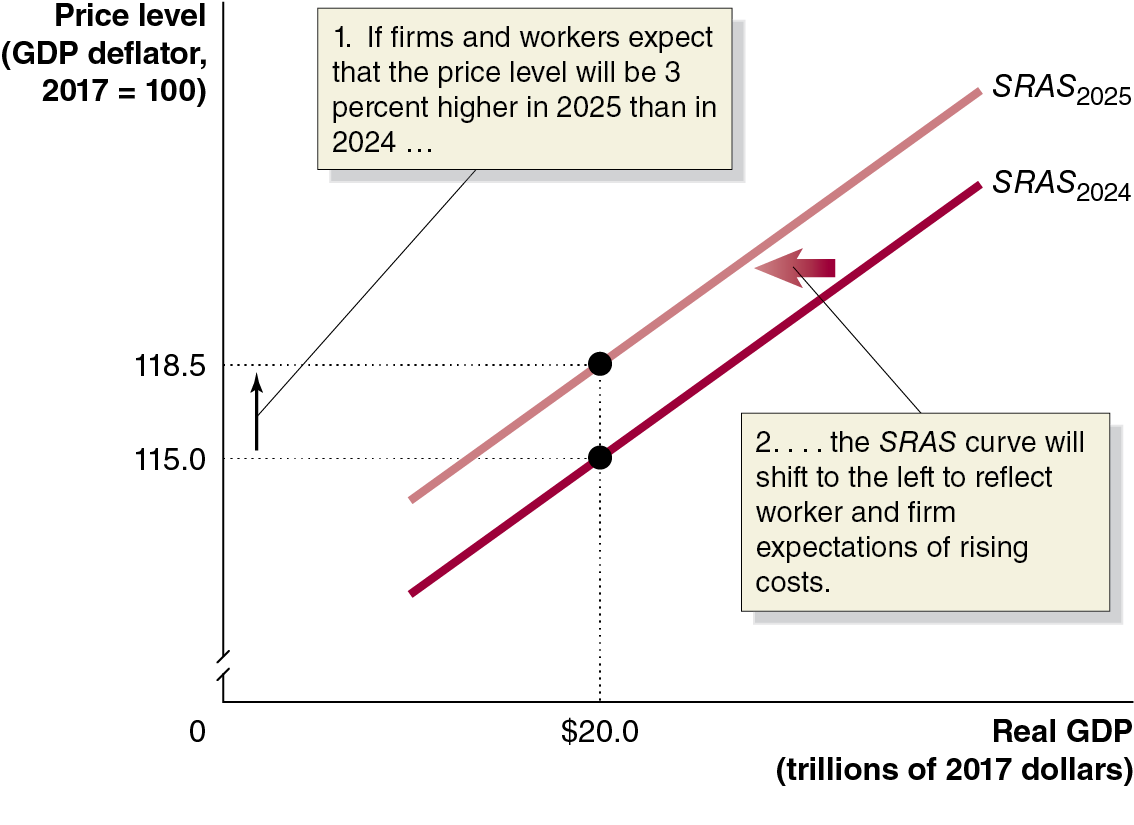
\includegraphics[width=\textwidth,height=0.99\textheight]{imgs3/img_slide26a.png}
\end{frame}

\begin{frame}{Table 13.2 Variables That Shift the Short-Run Aggregate
Supply Curve (1 of 3)}
\protect\hypertarget{table-13.2-variables-that-shift-the-short-run-aggregate-supply-curve-1-of-3}{}
Table 13.2 Variables That Shift the Short-Run Aggregate Supply Curve (1
of 3)

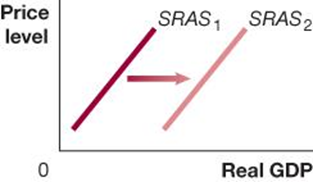
\includegraphics[width=\textwidth,height=0.99\textheight]{imgs3/img_slide27a.png}

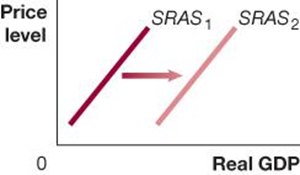
\includegraphics[width=\textwidth,height=0.99\textheight]{imgs3/img_slide27b.png}

An increase in the availability of the factors of production, i.e.~labor
and capital, allows more production at any price level. + A decrease in
the availability of these factors decreases S R A S.

Improvements in technology allow productivity to improve, and hence the
level of production at any given price level.
\end{frame}

\begin{frame}{Table 13.2 Variables That Shift the Short-Run Aggregate
Supply Curve (2 of 3)}
\protect\hypertarget{table-13.2-variables-that-shift-the-short-run-aggregate-supply-curve-2-of-3}{}
Table 13.2 Variables That Shift the Short-Run Aggregate Supply Curve (2
of 3)

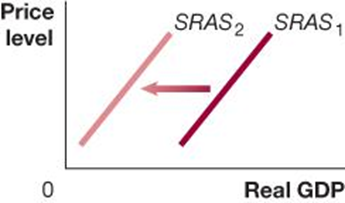
\includegraphics[width=\textwidth,height=0.99\textheight]{imgs3/img_slide28a.png}

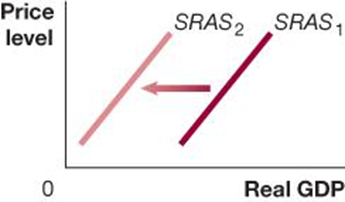
\includegraphics[width=\textwidth,height=0.99\textheight]{imgs3/img_slide28b.png}

If workers and firms expect higher prices in the future, S R A S shifts
to the left. This could happen because: + Inflation expectations
increase or + Workers and firms realize they previously underestimated
the price level.
\end{frame}

\begin{frame}{Table 13.2 Variables That Shift the Short-Run Aggregate
Supply Curve (3 of 3)}
\protect\hypertarget{table-13.2-variables-that-shift-the-short-run-aggregate-supply-curve-3-of-3}{}
Table 13.2 Variables That Shift the Short-Run Aggregate Supply Curve (3
of 3)

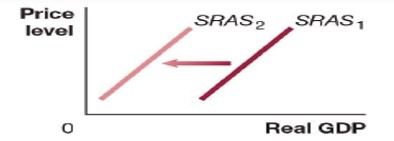
\includegraphics[width=\textwidth,height=0.99\textheight]{imgs3/img_slide29a.png}

A supply shock is an unexpected event that causes the short-run
aggregate supply curve to shift. + Examples: Oil prices increase
suddenly. Firms immediately anticipate rising input prices and will only
produce the same amount of output if their own prices rise. The pandemic
shutdown closed businesses and reduced supply in 2020. + Unexpected
input price increases cause a decrease in the S R A S; unexpected input
price decreases would shift S R A S to the right instead.
\end{frame}

\begin{frame}{13.3 Macroeconomic Equilibrium in the Long Run and the
Short Run}
\protect\hypertarget{macroeconomic-equilibrium-in-the-long-run-and-the-short-run}{}
13.3 Macroeconomic Equilibrium in the Long Run and the Short Run

Use the aggregate demand and aggregate supply model to illustrate the
difference between short-run and long-run macroeconomic equilibrium.

Now we are ready to introduce the long-run aggregate supply curve into
our model. + Remember, the L R A S shows the level of potential, or
full-employment, G D P.
\end{frame}

\begin{frame}{Figure 13.4 Long-Run Macroeconomic Equilibrium}
\protect\hypertarget{figure-13.4-long-run-macroeconomic-equilibrium}{}
Figure 13.4 Long-Run Macroeconomic Equilibrium

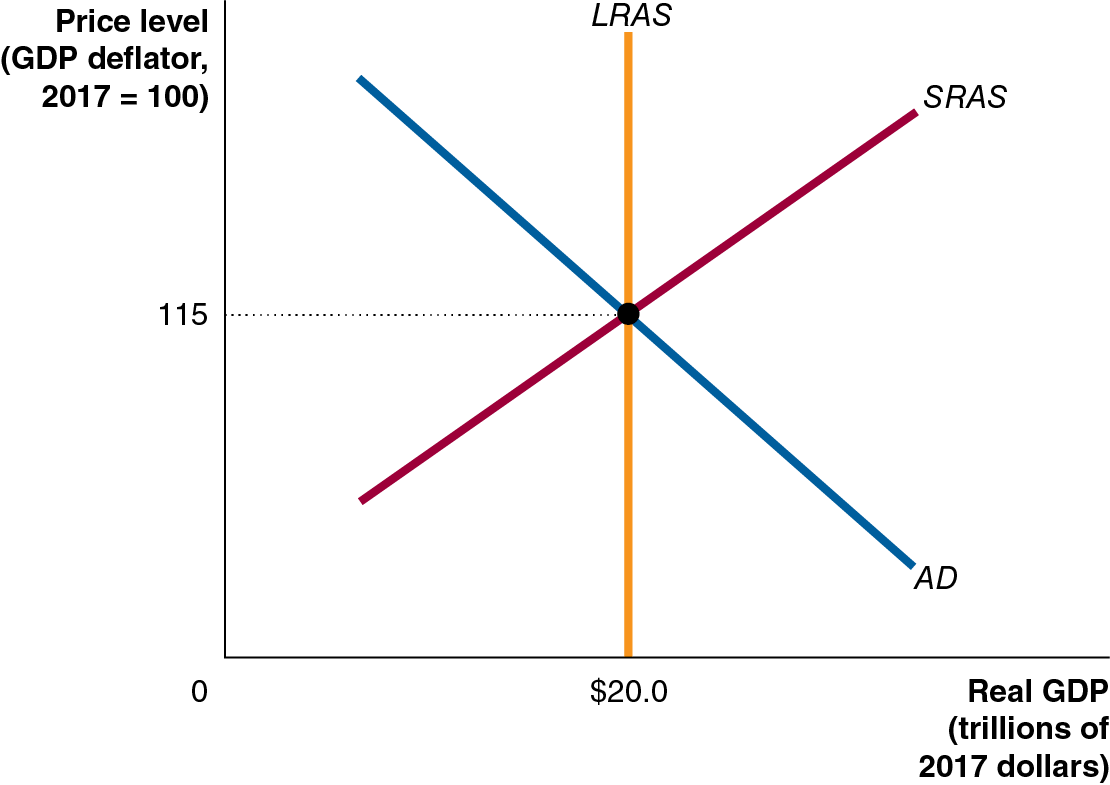
\includegraphics[width=\textwidth,height=0.99\textheight]{imgs3/img_slide31a.png}

Long-run macroeconomic equilibrium occurs when the A D and S R A S
curves intersect at the L R A S level, that is, when the economy is in
short-run equilibrium, and G D P is at its full-employment level. + For
simplicity, assume no inflation (current and expected price level is
115) and no growth (L R A S fixed at \$20.0 trillion).
\end{frame}

\begin{frame}{Figure 13.5 The Short-Run and Long-Run Effects of a
Decrease in Aggregate Demand (1 of 2)}
\protect\hypertarget{figure-13.5-the-short-run-and-long-run-effects-of-a-decrease-in-aggregate-demand-1-of-2}{}
Figure 13.5 The Short-Run and Long-Run Effects of a Decrease in
Aggregate Demand (1 of 2)

Suppose interest rates rise. + Planned investments fall: A D shifts
left, and the short-run macroeconomic equilibrium moves from A to B. +
Workers lose their jobs, firms lose sales: a recession

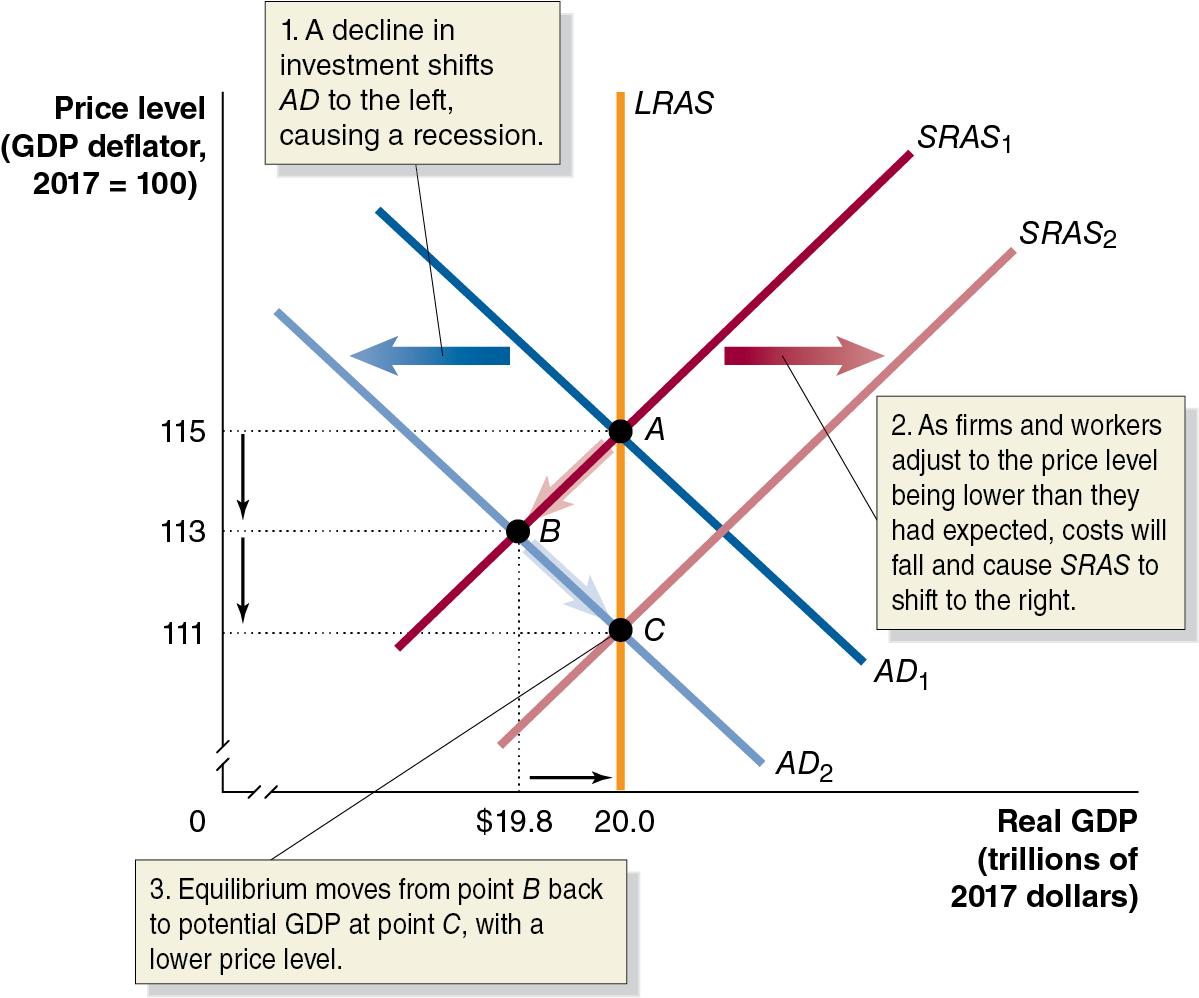
\includegraphics[width=\textwidth,height=0.99\textheight]{imgs3/img_slide32a.png}
\end{frame}

\begin{frame}{Figure 13.5 The Short-Run and Long-Run Effects of a
Decrease in Aggregate Demand (2 of 2)}
\protect\hypertarget{figure-13.5-the-short-run-and-long-run-effects-of-a-decrease-in-aggregate-demand-2-of-2}{}
Figure 13.5 The Short-Run and Long-Run Effects of a Decrease in
Aggregate Demand (2 of 2)

Workers accept lower wages and firms expect lower prices, including
lower input costs: S R A S shifts right, moving the short-run
macroeconomic equilibrium from B to C. + S R A S shifting right restores
long-run macroeconomic equilibrium, with a lower price level.

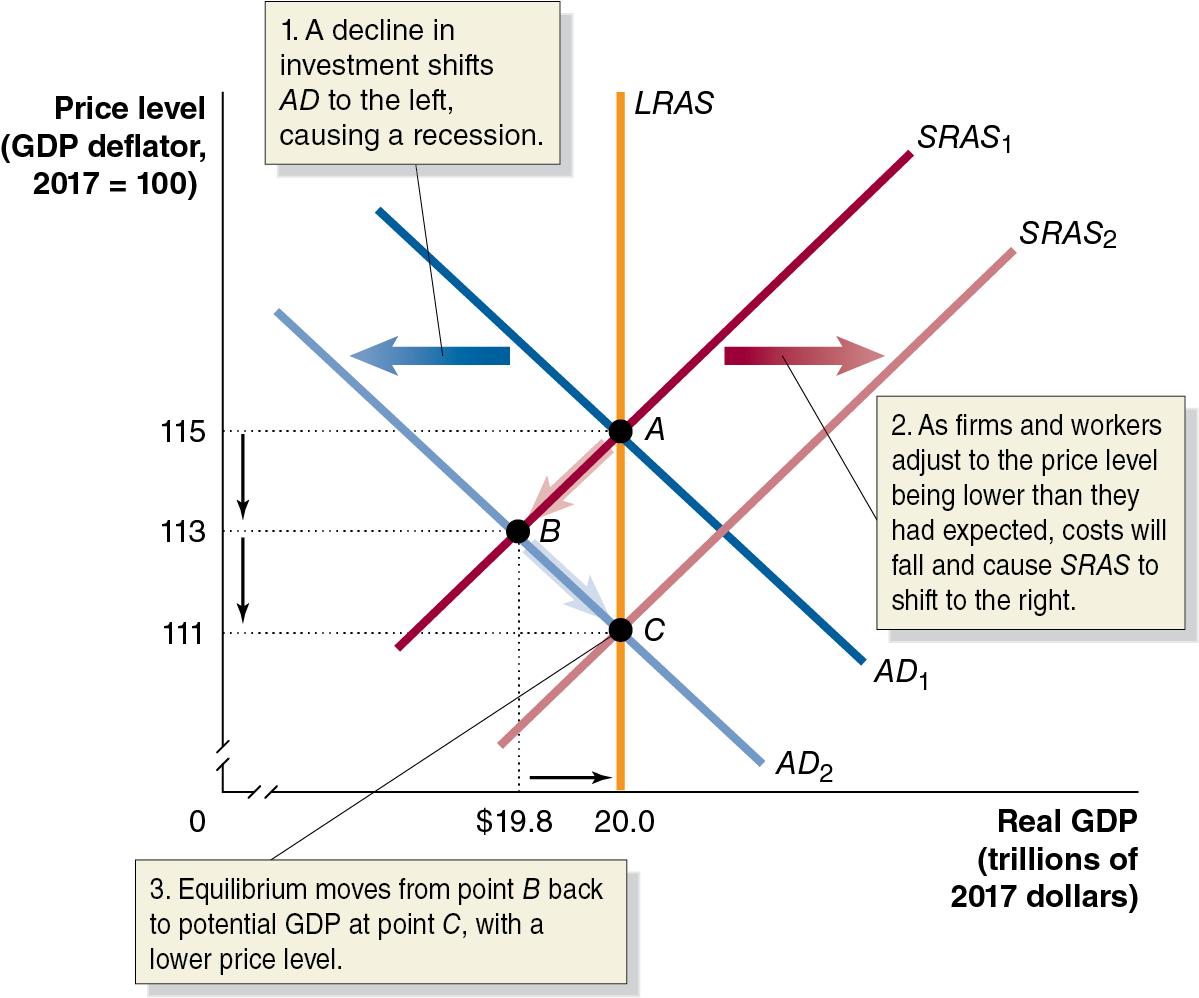
\includegraphics[width=\textwidth,height=0.99\textheight]{imgs3/img_slide33a.png}
\end{frame}

\begin{frame}{Apply the Concept: Does It Matter What Causes a Decline in
Aggregate Demand?}
\protect\hypertarget{apply-the-concept-does-it-matter-what-causes-a-decline-in-aggregate-demand}{}
Apply the Concept: Does It Matter What Causes a Decline in Aggregate
Demand?

G D P has four components; a decrease in any of the four could cause a
recession. Does it make any difference which component causes the
recession?

Ed Leamer of U C L A: ``housing is the business cycle.'' + Recent
research suggests that recessions caused by financial crises tend to be
larger and more long-lasting than declines due to other factors.


\includegraphics[width=\textwidth,height=0.99\textheight]{imgs3/img_slide34a.png}
\end{frame}

\begin{frame}{Figure 13.6 The Short-Run and Long-Run Effects of an
Increase in Aggregate Demand (1 of 2)}
\protect\hypertarget{figure-13.6-the-short-run-and-long-run-effects-of-an-increase-in-aggregate-demand-1-of-2}{}
Figure 13.6 The Short-Run and Long-Run Effects of an Increase in
Aggregate Demand (1 of 2)

Suppose that firms become more optimistic about the future. + They
increase investment, shifting A D to the right, shifting the short-run
macroeconomic equilibrium from A to B. + Unemployment falls below its
natural rate, raising wages; the increased demand for goods raises
prices.

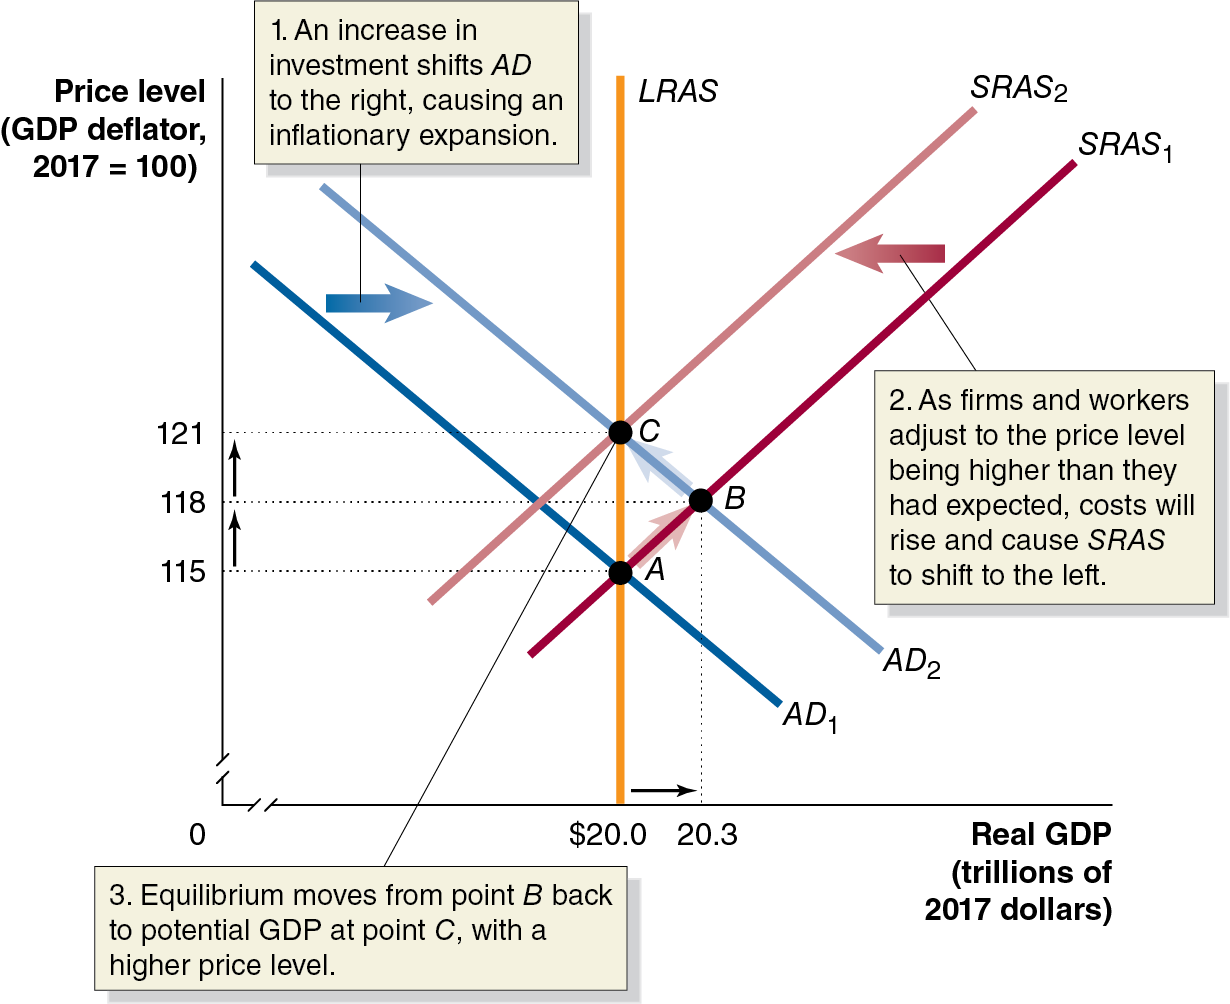
\includegraphics[width=\textwidth,height=0.99\textheight]{imgs3/img_slide35a.png}
\end{frame}

\begin{frame}{Figure 13.6 The Short-Run and Long-Run Effects of an
Increase in Aggregate Demand (2 of 2)}
\protect\hypertarget{figure-13.6-the-short-run-and-long-run-effects-of-an-increase-in-aggregate-demand-2-of-2}{}
Figure 13.6 The Short-Run and Long-Run Effects of an Increase in
Aggregate Demand (2 of 2)

Firms and workers raise expectations about the price level, shifting S R
A S to the left---restoring long- run macroeconomic equilibrium at point
C.

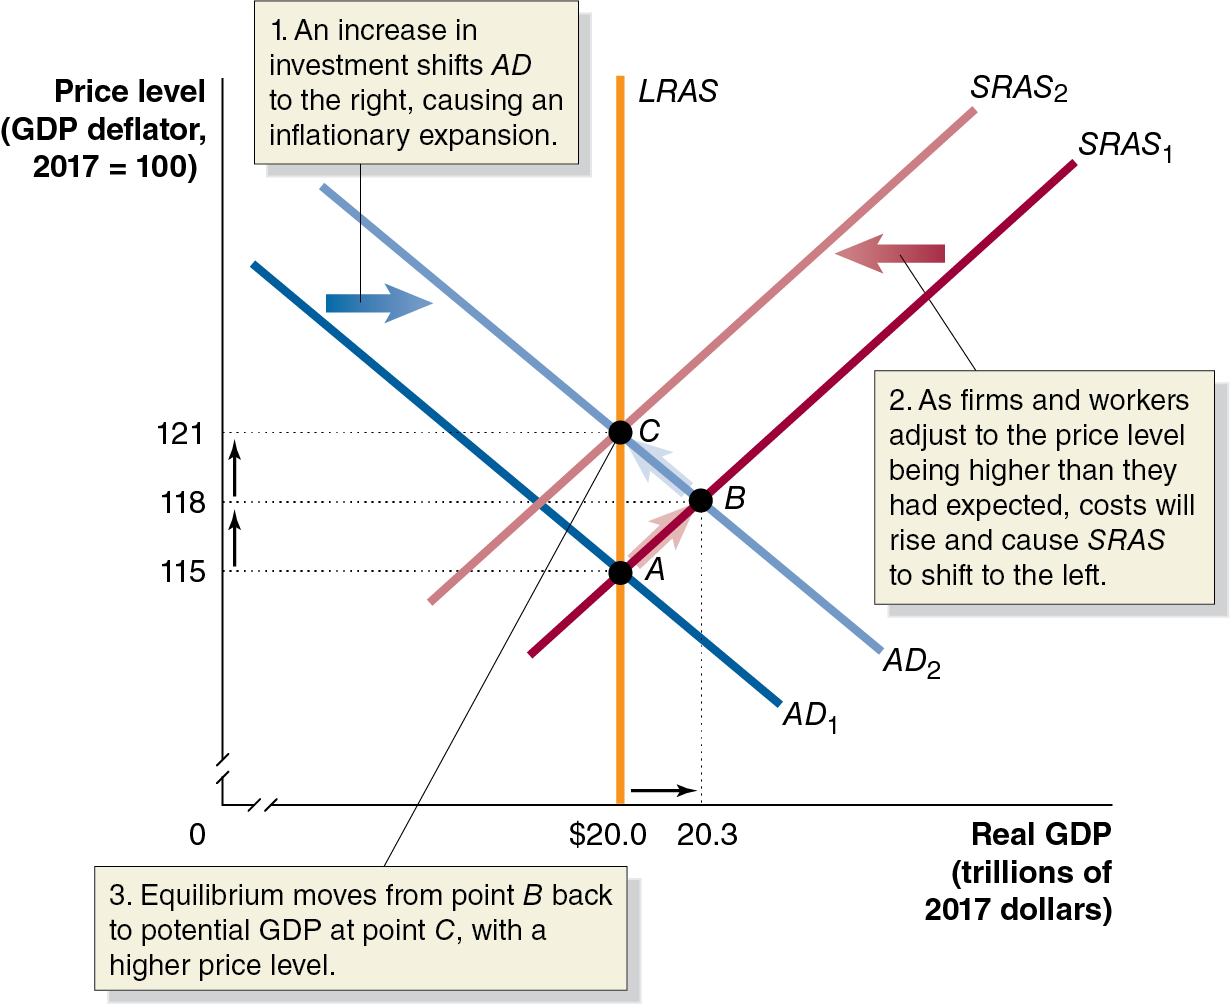
\includegraphics[width=\textwidth,height=0.99\textheight]{imgs3/img_slide36a.png}
\end{frame}

\begin{frame}{Figure 13.7 The Short-Run and Long-Run Effects of a Supply
Shock (1 of 3)}
\protect\hypertarget{figure-13.7-the-short-run-and-long-run-effects-of-a-supply-shock-1-of-3}{}
Figure 13.7 The Short-Run and Long-Run Effects of a Supply Shock (1 of
3)

In the previous analyses, A D moved suddenly. What if instead S R A S
moved suddenly? We call this a supply shock. + For example, suppose a
sudden increase in oil prices shifts S R A S to the left. + This causes
stagflation, a combination of inflation and recession, usually resulting
from a supply shock.

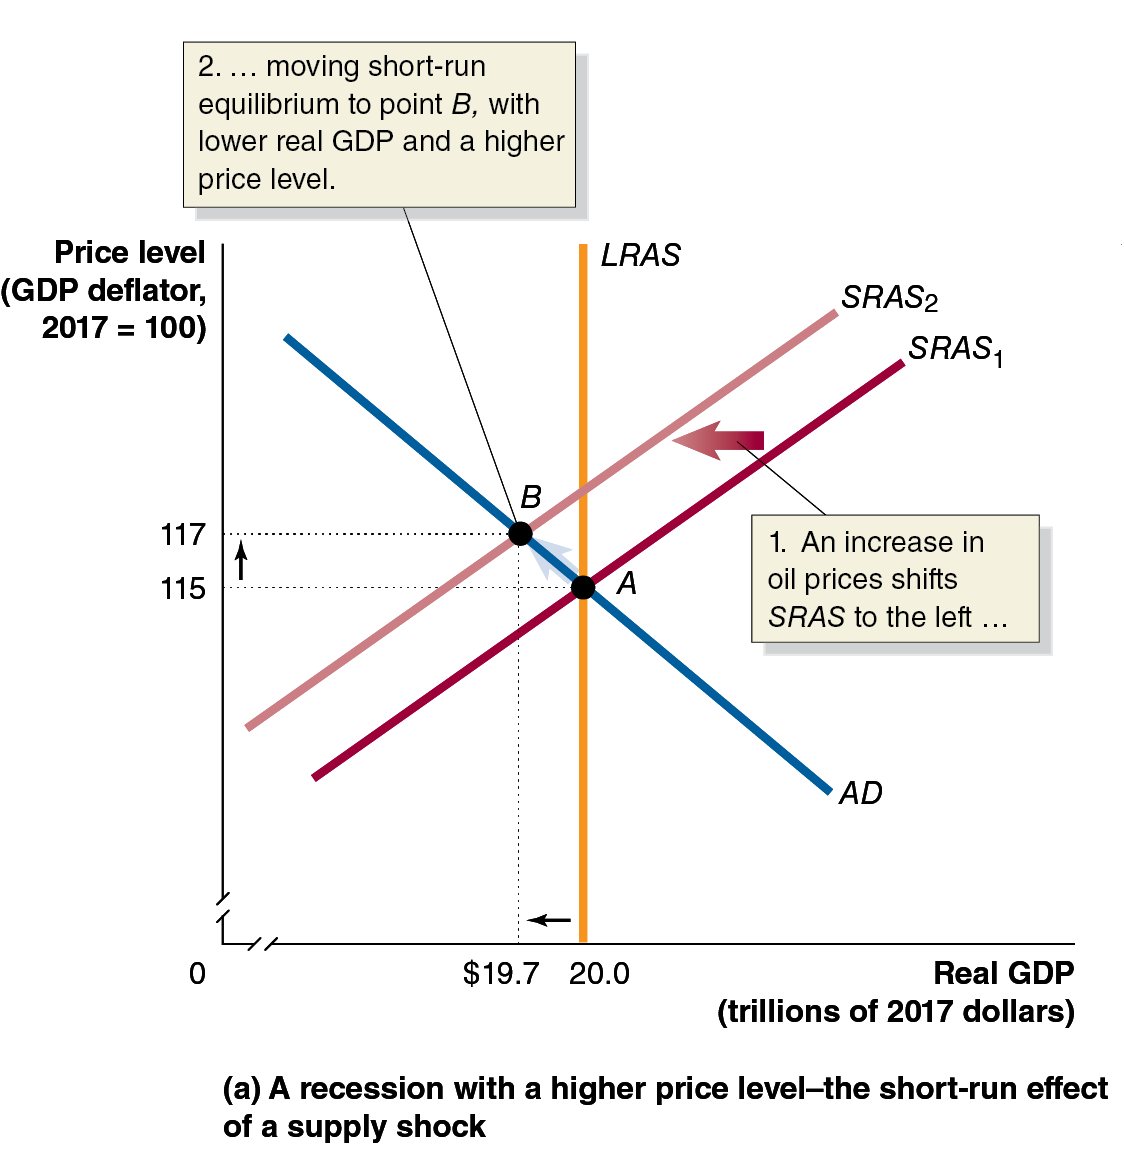
\includegraphics[width=\textwidth,height=0.99\textheight]{imgs3/img_slide37a.png}
\end{frame}

\begin{frame}{Figure 13.7 The Short-Run and Long-Run Effects of a Supply
Shock (2 of 3)}
\protect\hypertarget{figure-13.7-the-short-run-and-long-run-effects-of-a-supply-shock-2-of-3}{}
Figure 13.7 The Short-Run and Long-Run Effects of a Supply Shock (2 of
3)

With the lower level of output, people are unemployed and products go
unsold. + Workers accept a lower wage, and firms decrease prices in
order to clear inventories. + With the decrease in expectations about
prices, S R A S moves to the right, restoring long-run equilibrium.

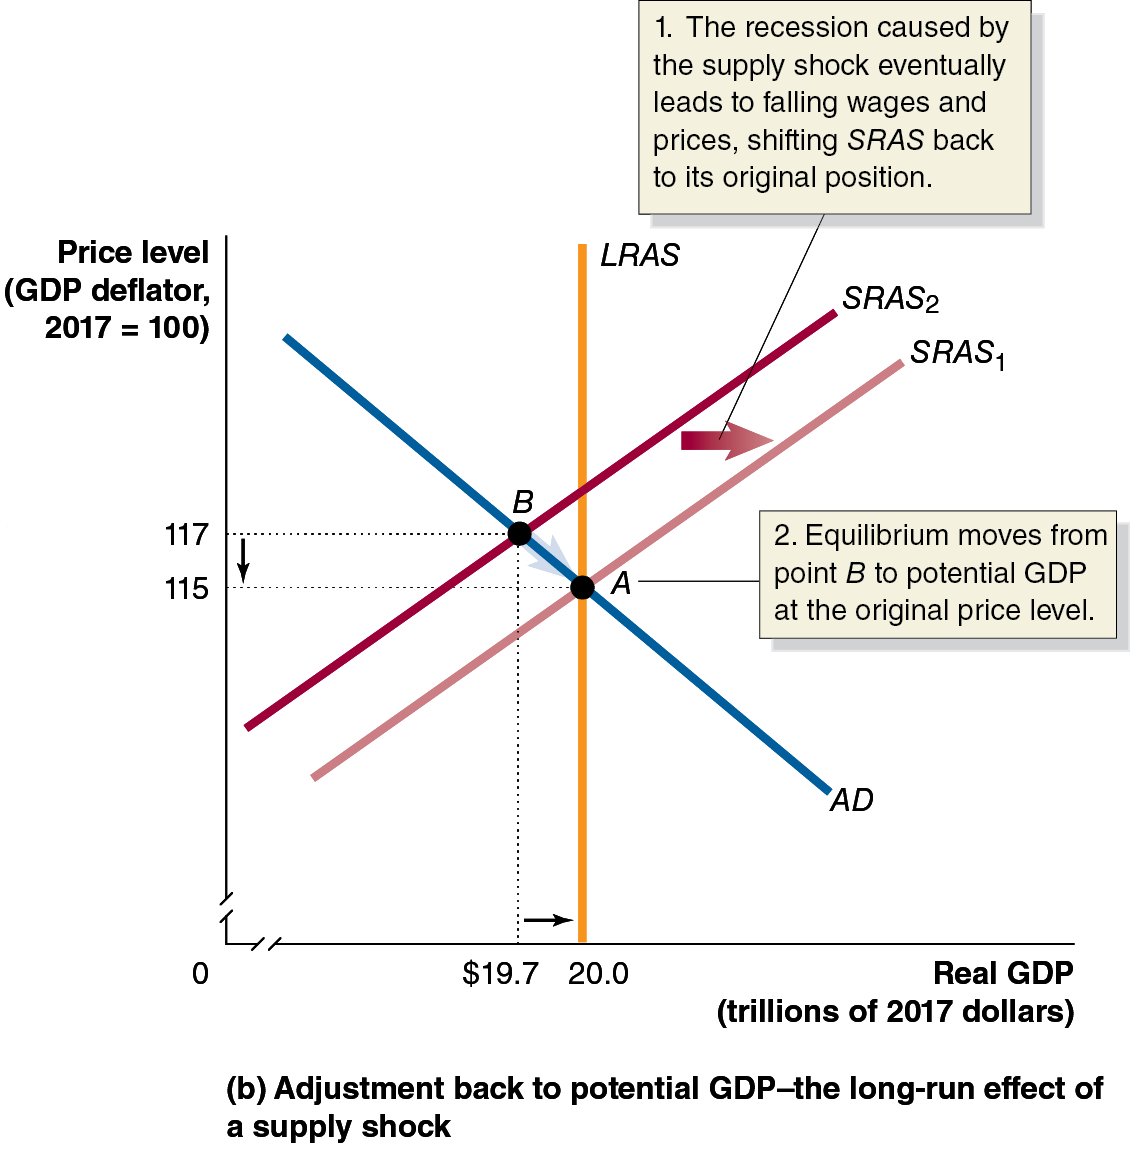
\includegraphics[width=\textwidth,height=0.99\textheight]{imgs3/img_slide38a.png}
\end{frame}

\begin{frame}{Figure 13.7 The Short-Run and Long-Run Effects of a Supply
Shock (3 of 3)}
\protect\hypertarget{figure-13.7-the-short-run-and-long-run-effects-of-a-supply-shock-3-of-3}{}
Figure 13.7 The Short-Run and Long-Run Effects of a Supply Shock (3 of
3)

How long does it take to restore full employment? + It depends on the
severity of the supply shock, but it is likely to take several years.

An alternative to waiting this long is to use fiscal or monetary policy
to increase aggregate demand. + This will result in permanently higher
prices but may be worth the cost.

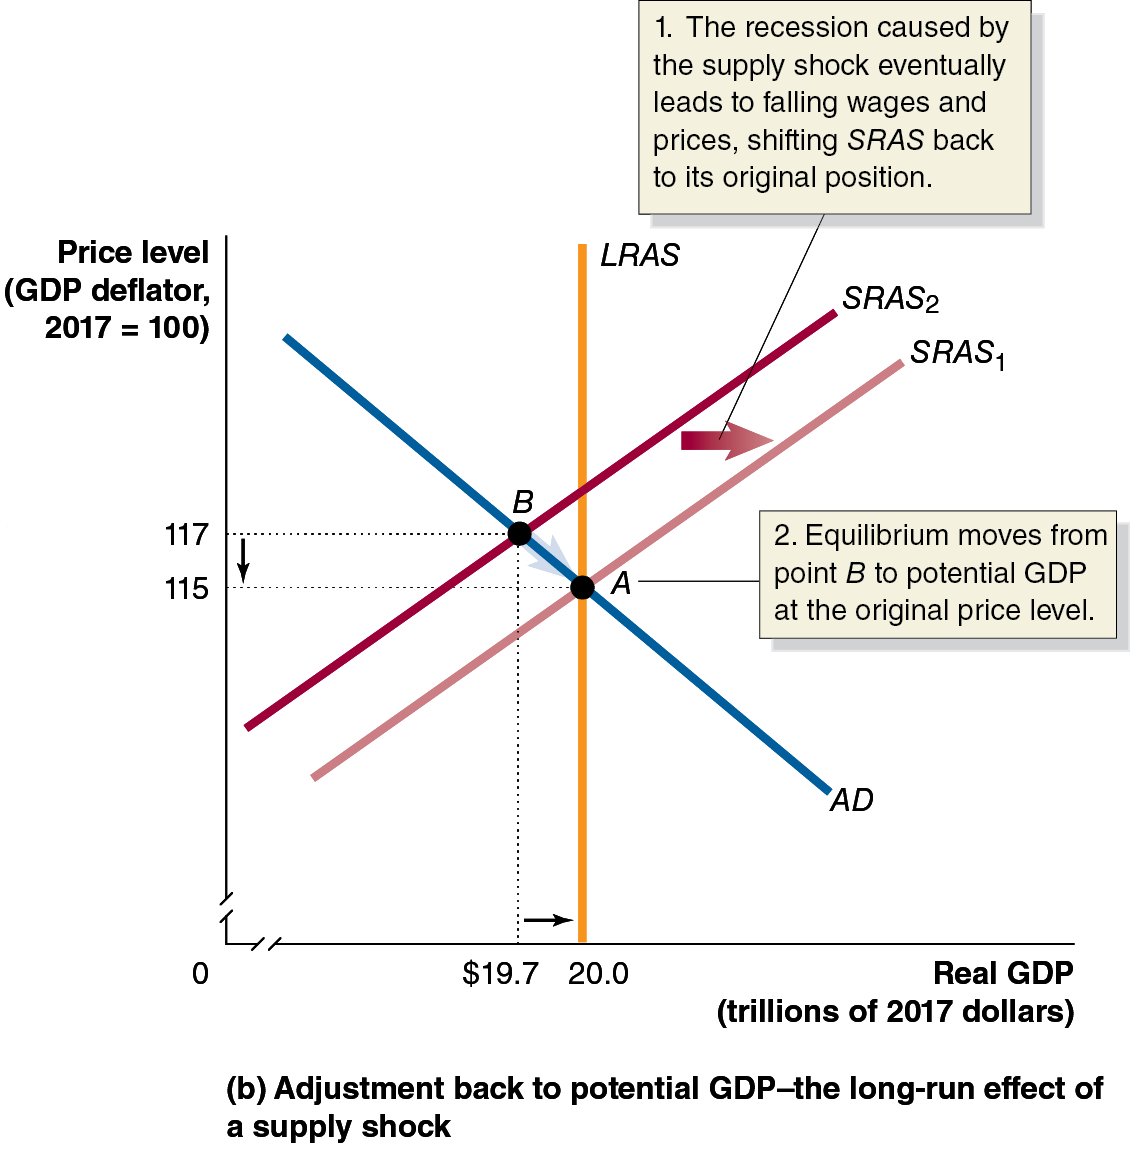
\includegraphics[width=\textwidth,height=0.99\textheight]{imgs3/img_slide39a.png}
\end{frame}

\begin{frame}{Figure 13.8 The Effects of the Covid-19 Pandemic}
\protect\hypertarget{figure-13.8-the-effects-of-the-covid-19-pandemic}{}
Figure 13.8 The Effects of the Covid-19 Pandemic

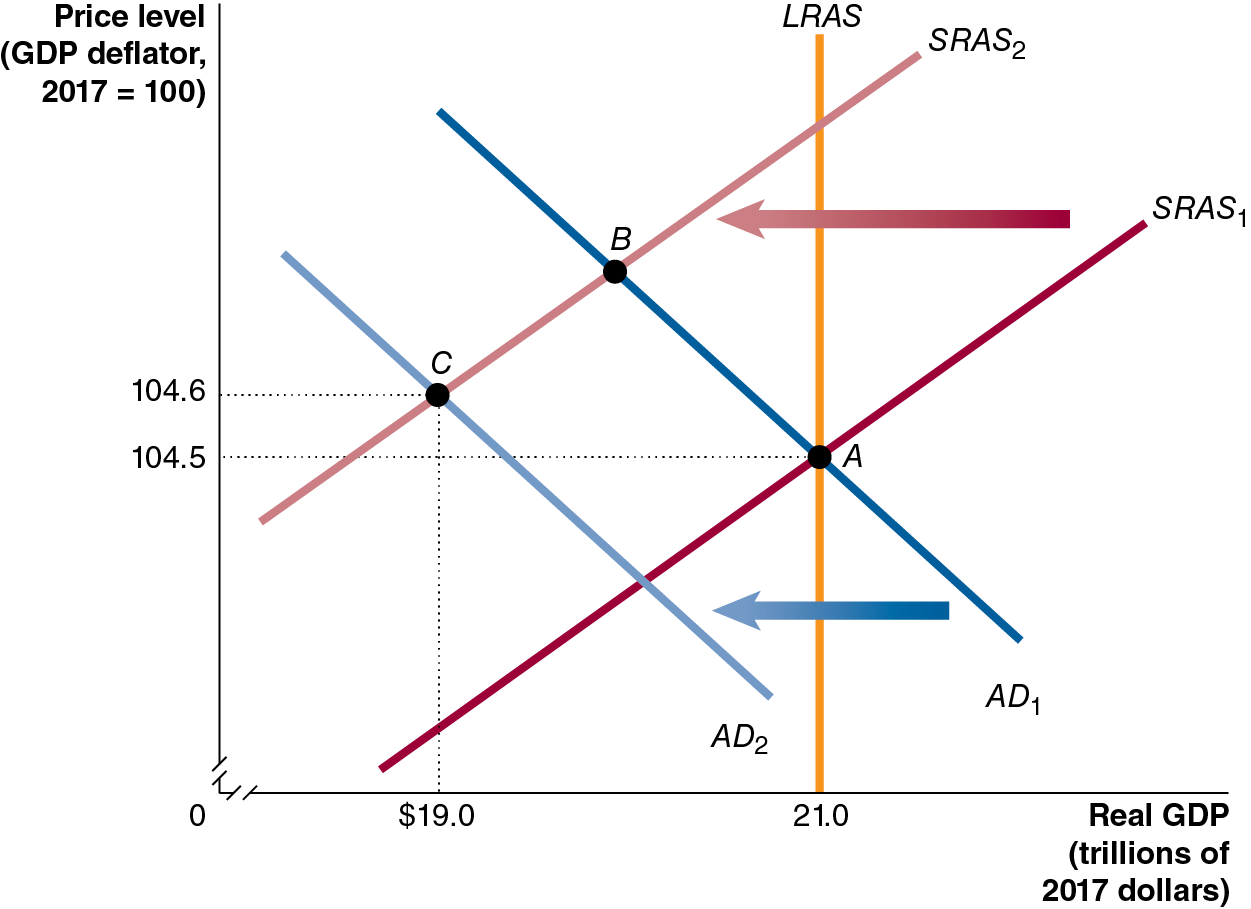
\includegraphics[width=\textwidth,height=0.99\textheight]{imgs3/img_slide40a.png}

Before the pandemic, the economy was in long-run equilibrium at Point A.
+ The pandemic created a supply shock, which would normally push the
short-run supply curve to the left and create a new equilibrium at Point
B. + However, the pandemic also affected A D resulting in a new
equilibrium at Point C.
\end{frame}

\begin{frame}{The Effects of the Covid-19 Pandemic}
\protect\hypertarget{the-effects-of-the-covid-19-pandemic}{}
The Effects of the Covid-19 Pandemic

Point B was not the new short-run equilibrium for three key reasons: +
Reduced consumption spending. State and local governments closed many
businesses, which directly reduced output and consumption spending,
particularly spending on services like restaurant meals and movie
tickets. + Reduced investment spending. Many residential and business
construction projects had to be suspended, reducing investment spending.
+ Reduced exports. U.S. exports declined because the pandemic also led
to closures of businesses in Europe, Canada, Japan, and other U.S.
trading partners.

Because the Covid-19 pandemic caused both the S R A S and A D curves to
shift to the left, the new short-run equilibrium occurred at point C,
with real G D P having fallen to \$19.0 trillion in the second quarter
of 2020, with prices approximately steady at 104.6.
\end{frame}

\begin{frame}{Apply the Concept: Is the Business Cycle Really a Cycle?
(1 of 2)}
\protect\hypertarget{apply-the-concept-is-the-business-cycle-really-a-cycle-1-of-2}{}
Apply the Concept: Is the Business Cycle Really a Cycle? (1 of 2)

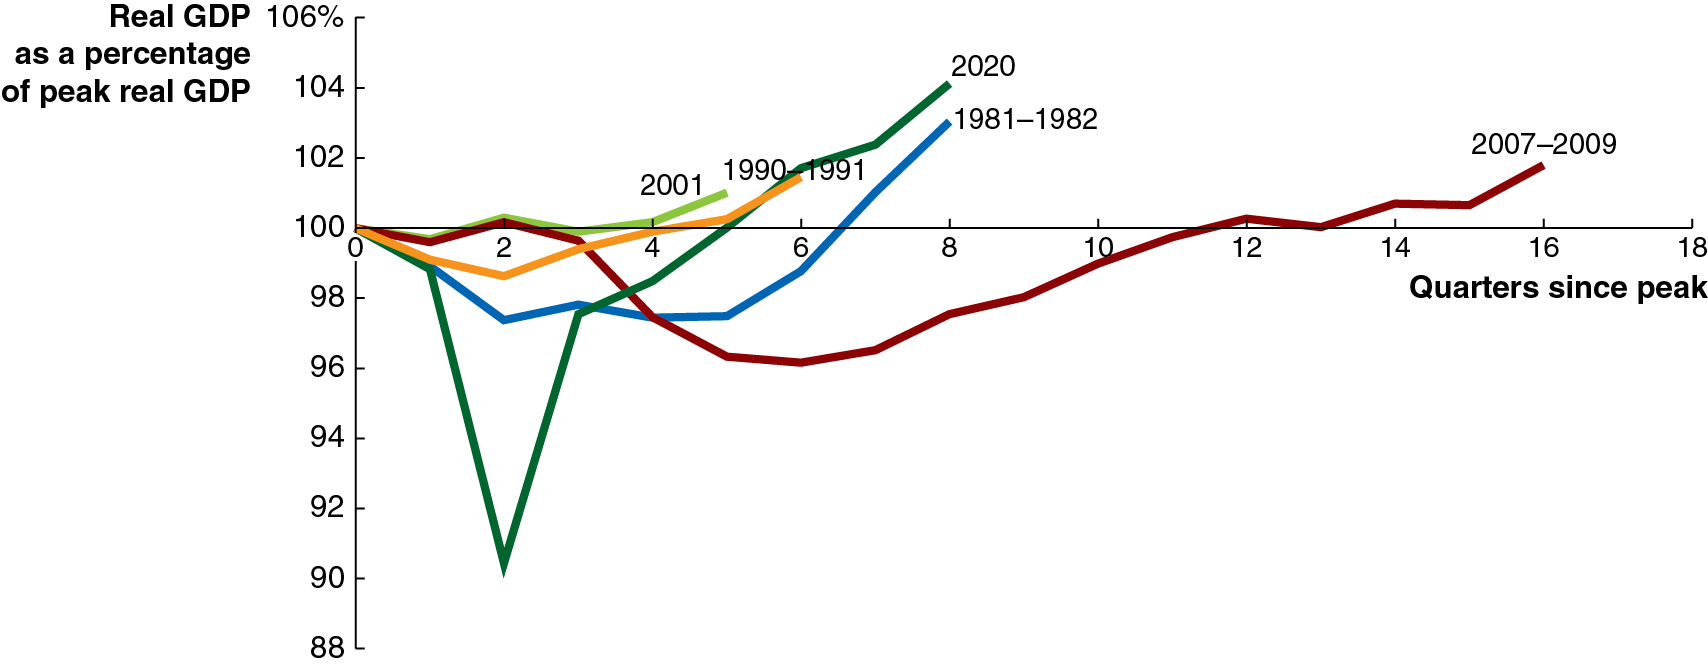
\includegraphics[width=\textwidth,height=0.99\textheight]{imgs3/img_slide42a.png}

The word cycle suggests a process that is uniform. + In the late 1800s,
some argued the business cycle was 11 years, the same as cycles in
sunspot activity. + This caused natural phenomena that drove the
business cycle.
\end{frame}

\begin{frame}{Apply the Concept: Is the Business Cycle Really a Cycle?
(2 of 2)}
\protect\hypertarget{apply-the-concept-is-the-business-cycle-really-a-cycle-2-of-2}{}
Apply the Concept: Is the Business Cycle Really a Cycle? (2 of 2)

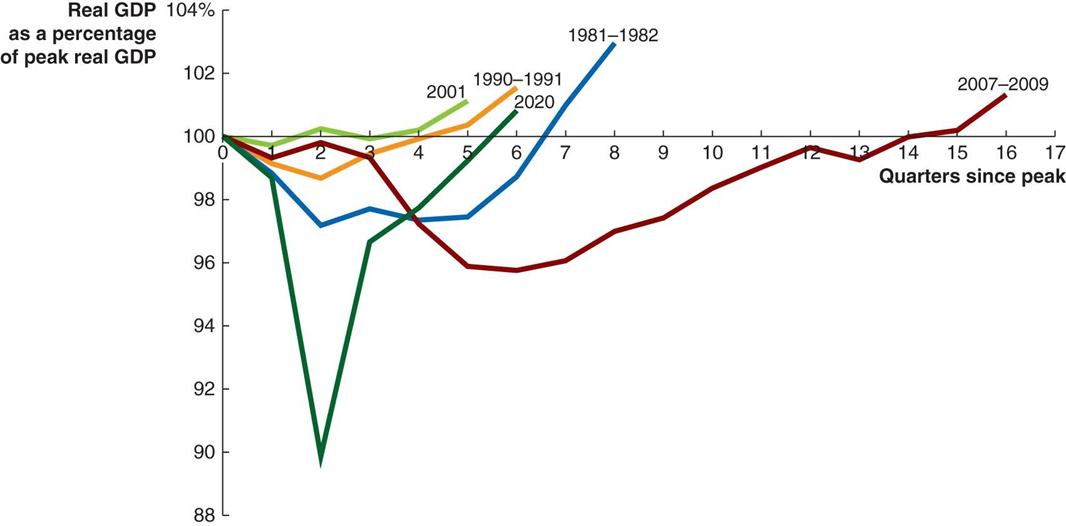
\includegraphics[width=\textwidth,height=0.99\textheight]{imgs3/img_slide43a.png}

It is clear now that business cycles vary greatly in length and
severity. + The graph shows how long the economy took to return to its
previous peak following each of the last five recessions.
\end{frame}

\begin{frame}{13.4 A Dynamic Aggregate Demand and Aggregate Supply
Model}
\protect\hypertarget{a-dynamic-aggregate-demand-and-aggregate-supply-model}{}
13.4 A Dynamic Aggregate Demand and Aggregate Supply Model

Use the dynamic aggregate demand and aggregate supply model to analyze
macroeconomic conditions.

Our model of aggregate demand and aggregate supply so far has been
static, in the sense that: + Price levels were constant (no inflation) +
There was no long-run growth

We will now form a dynamic aggregate demand and aggregate supply model,
incorporating: + Continually increasing real G D P, shifting L R A S to
the right + A D also ordinarily shifting to the right + S R A S shifting
to the right, except when workers and firms expect high rates of
inflation
\end{frame}

\begin{frame}{Figure 13.9 A Dynamic Aggregate Demand and Aggregate
Supply Model}
\protect\hypertarget{figure-13.9-a-dynamic-aggregate-demand-and-aggregate-supply-model}{}
Figure 13.9 A Dynamic Aggregate Demand and Aggregate Supply Model

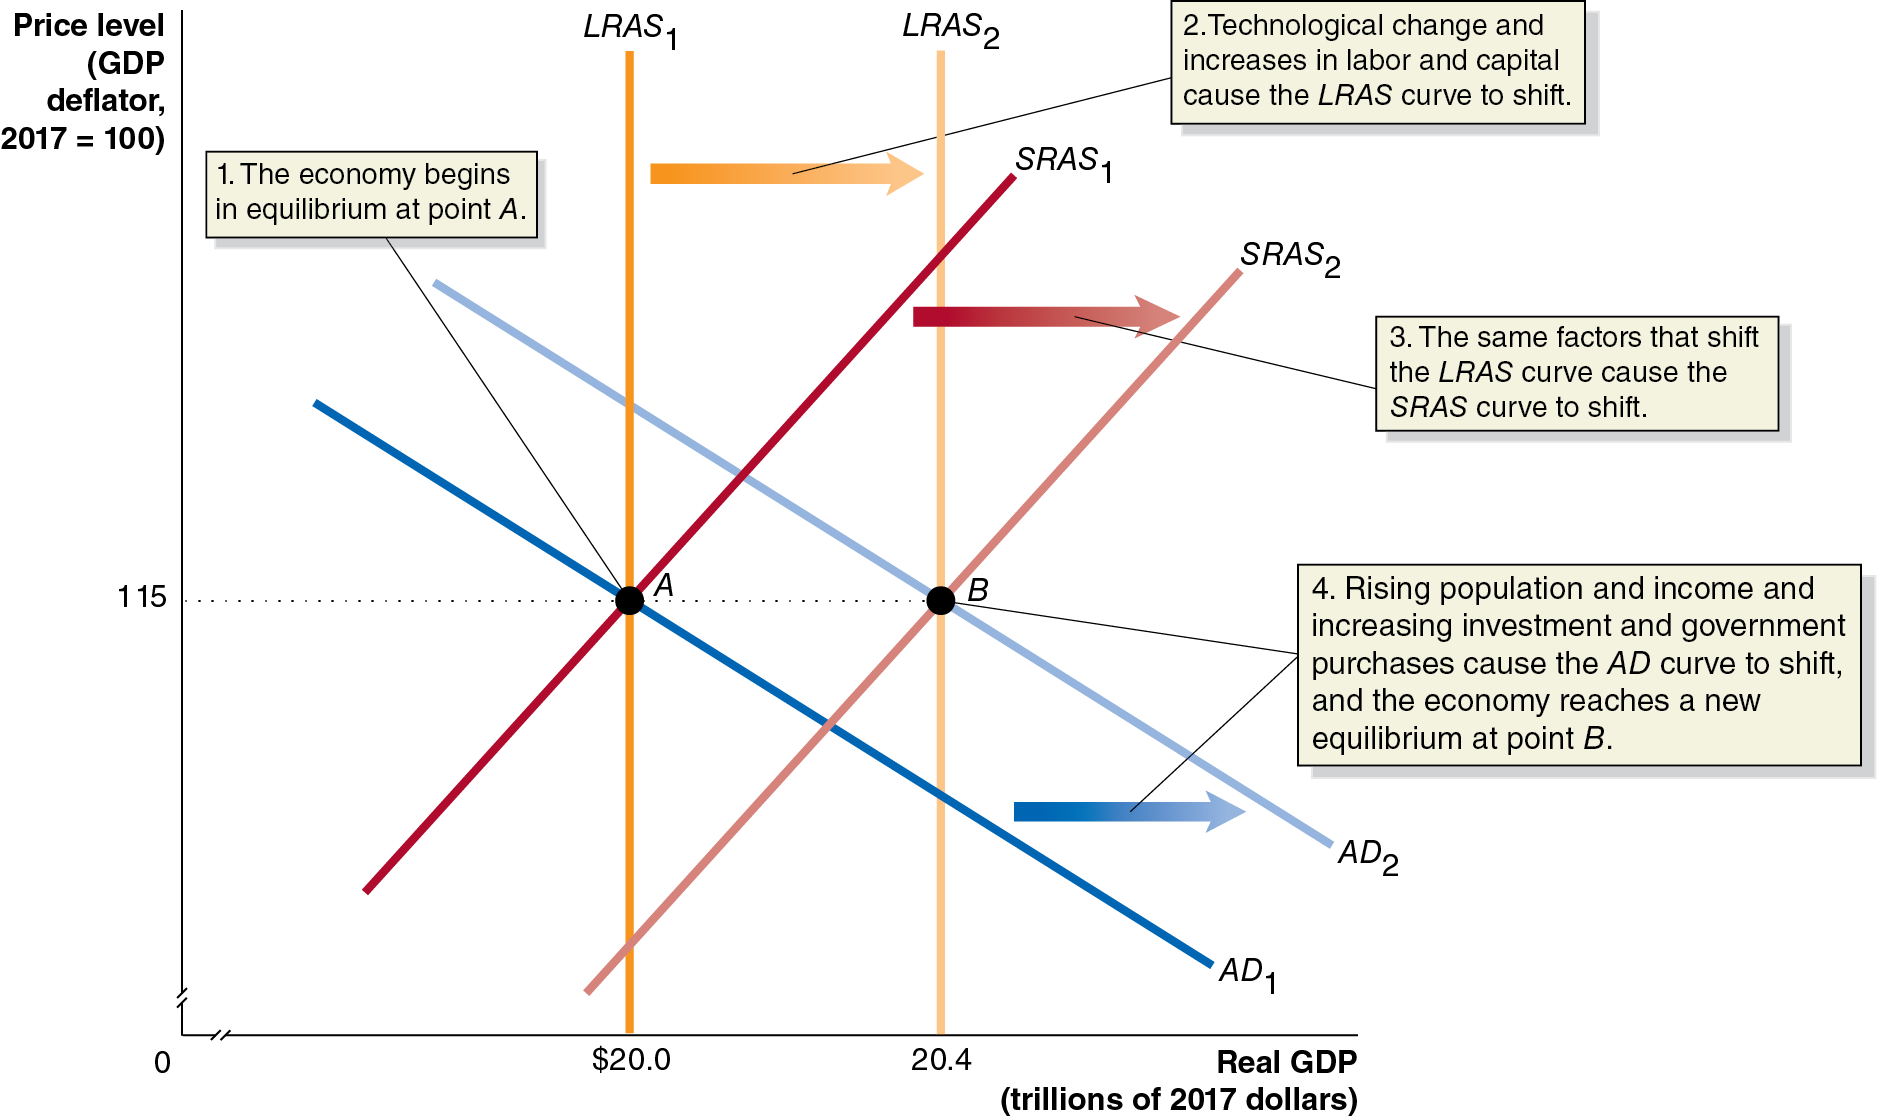
\includegraphics[width=\textwidth,height=0.99\textheight]{imgs3/img_slide45a.png}
\end{frame}

\begin{frame}{Figure 13.10 Using Dynamic Aggregate Demand and Aggregate
Supply to Understand Inflation}
\protect\hypertarget{figure-13.10-using-dynamic-aggregate-demand-and-aggregate-supply-to-understand-inflation}{}
Figure 13.10 Using Dynamic Aggregate Demand and Aggregate Supply to
Understand Inflation

The usual cause of inflation is total spending increasing faster than
production. + A D moves further right than does L R A S. + S R A S moves
to the right; but the anticipated rise in the price level causes it to
shift less than L R A S. + Long-run equilibrium is restored but with a
higher price level.

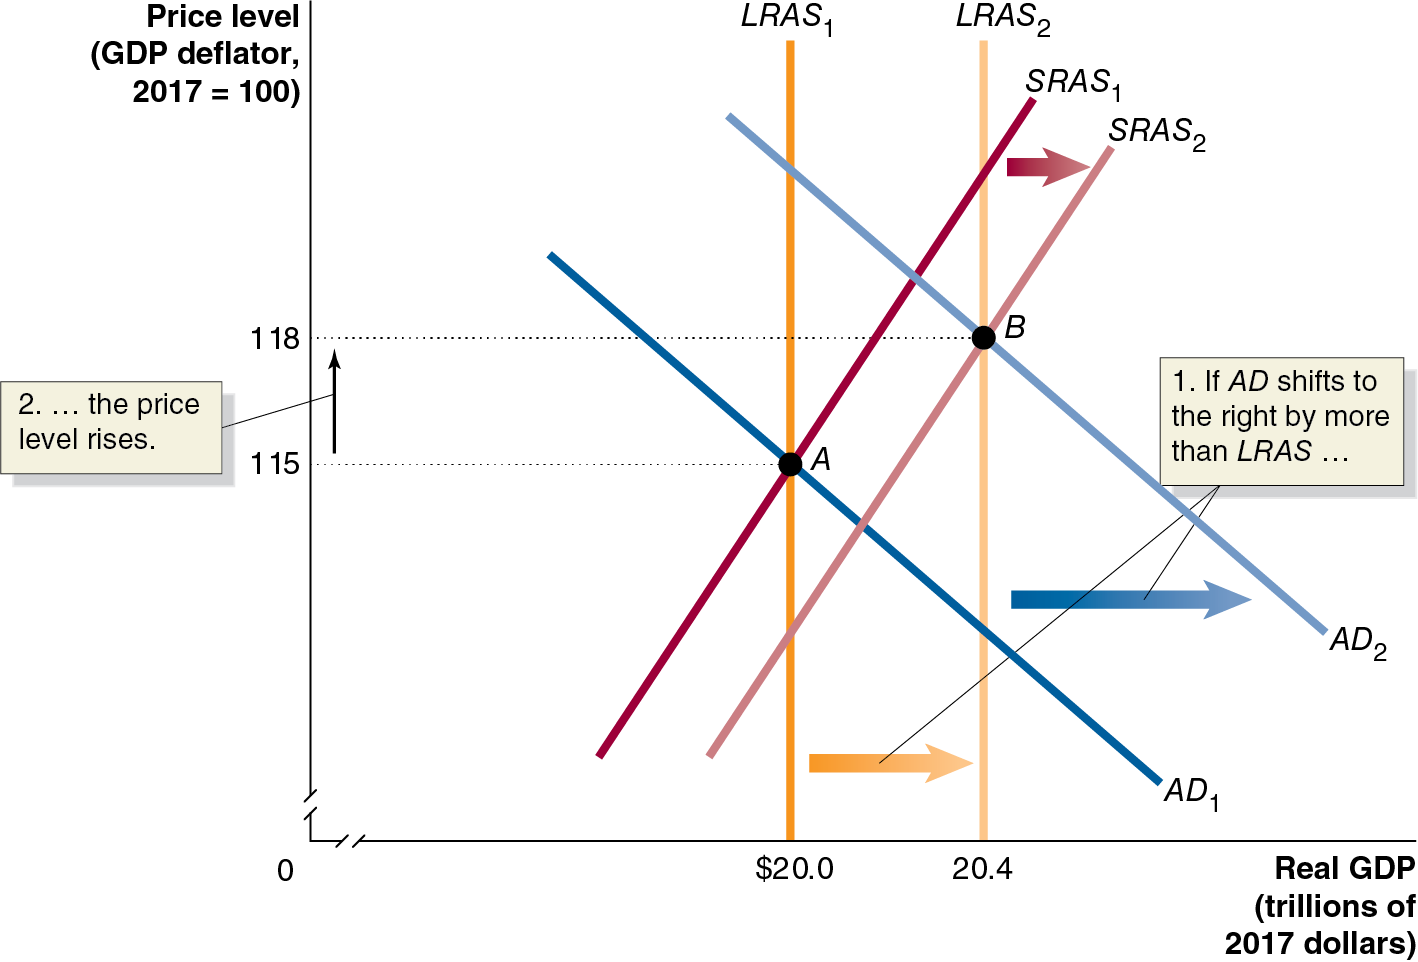
\includegraphics[width=\textwidth,height=0.99\textheight]{imgs3/img_slide46a.png}
\end{frame}

\begin{frame}{Main Factors Causing the Recession of 2007--2009}
\protect\hypertarget{main-factors-causing-the-recession-of-20072009}{}
Main Factors Causing the Recession of 2007--2009

The end of the housing bubble

House prices rose in the early 2000s---initially due to low interest
rates, but then due to speculation. In 2006, the speculative bubble
began to deflate, and the spending on residential investment fell.

The 2007--2009 financial crisis

As many people defaulted on their mortgages, many financial institutions
took heavy losses. This financial crisis led to a credit crunch,
decreasing consumption and investment spending.

The rapid increase in oil prices during 2008

Several factors combined to increase the price of oil from \$34 per
barrel in 2004 to \$140 per barrel in mid-2008. This supply shock
exacerbated the ongoing recession.
\end{frame}

\begin{frame}{Figure 13.11 The Recession of 2007--2009 (1 of 2)}
\protect\hypertarget{figure-13.11-the-recession-of-20072009-1-of-2}{}
Figure 13.11 The Recession of 2007--2009 (1 of 2)

In 2007, the economy was a little below long-run equilibrium. + As
usual, potential G D P increased from 2007 to 2009. + But aggregate
demand did not keep pace (housing bubble, financial crisis).

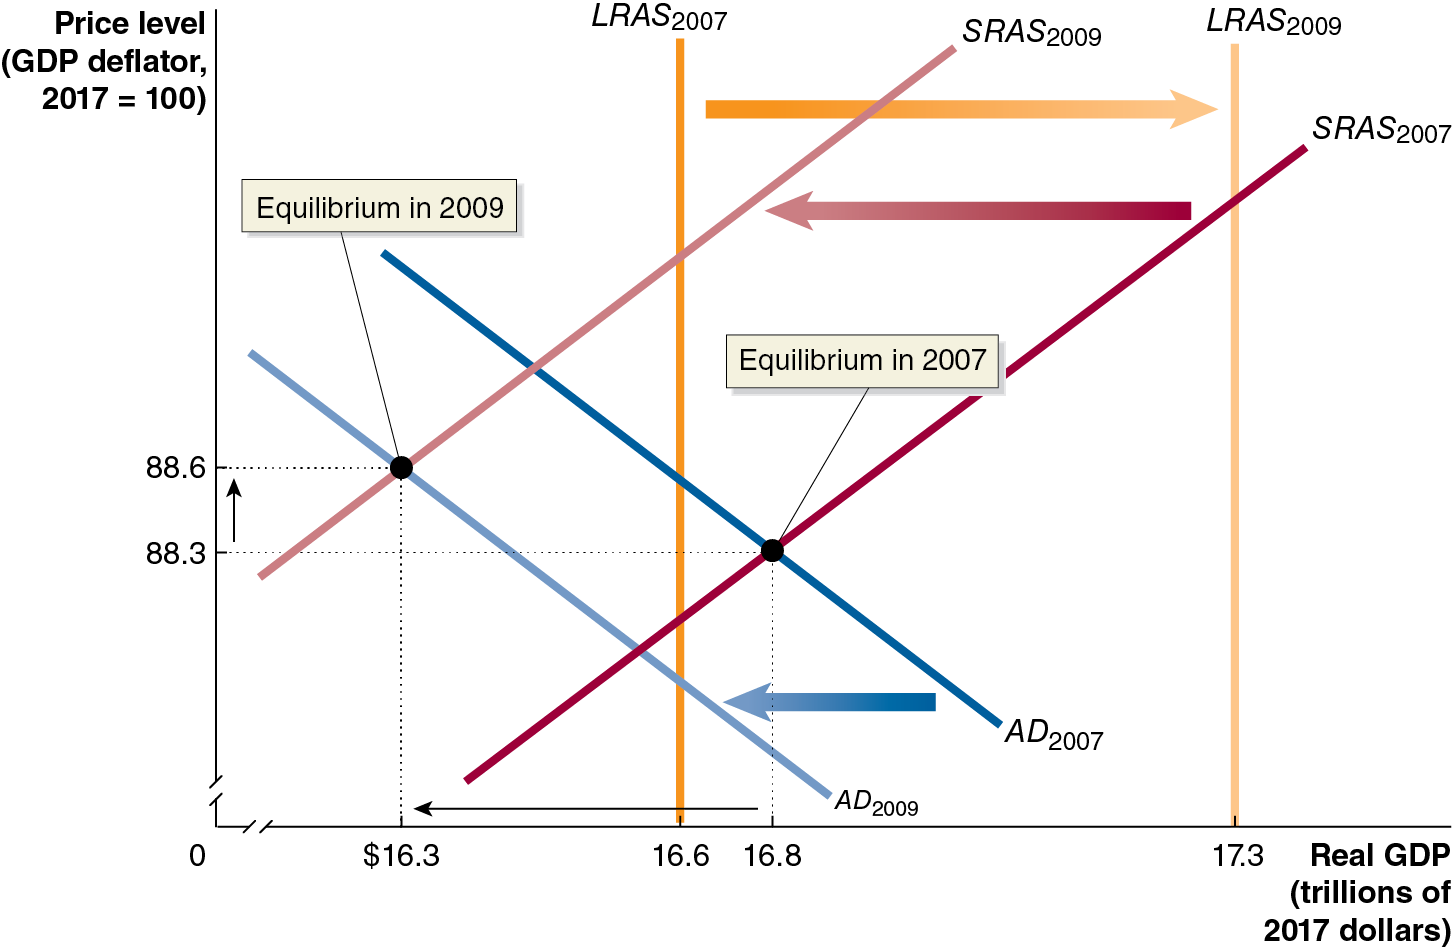
\includegraphics[width=\textwidth,height=0.99\textheight]{imgs3/img_slide48a.png}
\end{frame}

\begin{frame}{Figure 13.11 The Recession of 2007--2009 (2 of 2)}
\protect\hypertarget{figure-13.11-the-recession-of-20072009-2-of-2}{}
Figure 13.11 The Recession of 2007--2009 (2 of 2)

At the same time, increasing oil prices shifted short-run aggregate
supply to the left. + The result: higher prices and real G D P that was
well below potential.

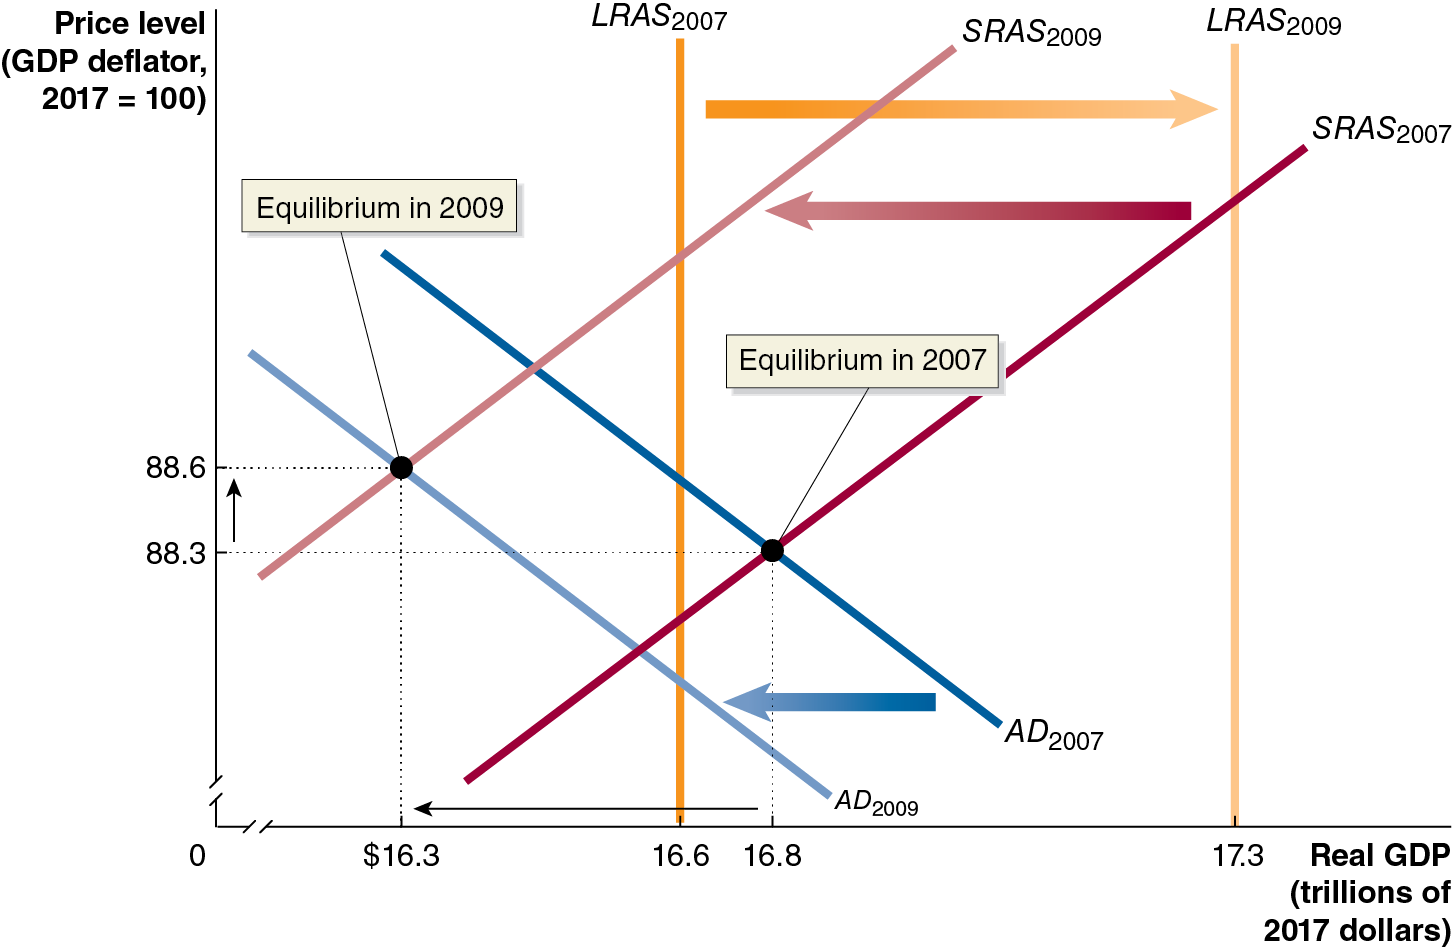
\includegraphics[width=\textwidth,height=0.99\textheight]{imgs3/img_slide49a.png}
\end{frame}

\begin{frame}{Appendix: Macroeconomic Schools of Thought}
\protect\hypertarget{appendix-macroeconomic-schools-of-thought}{}
Appendix: Macroeconomic Schools of Thought

Compare macroeconomic schools of thought.

Macroeconomic theory is relatively less settled than microeconomic
theory. + Macroeconomics developed as a separate field within economics
after the Great Depression. + John Maynard Keynes's 19 36 book The
General Theory of Employment, Interest, and Money inspires the model we
have addressed in this chapter. + Widespread acceptance during the 19
30s and 19 40s of Keynes's model became known as the Keynesian
revolution.
\end{frame}

\begin{frame}{New Keynesian Economics}
\protect\hypertarget{new-keynesian-economics}{}
New Keynesian Economics

Modern followers of Keynes refer to themselves as new Keynesians. +
Emphasize the stickiness of wages and prices in explaining fluctuations
in real G D P---a concept that Keynes did not include in his original
model.
\end{frame}

\begin{frame}{The Monetarist Model}
\protect\hypertarget{the-monetarist-model}{}
The Monetarist Model

Monetarism refers to the macroeconomic theories of Milton Friedman and
his followers, particularly the idea that the quantity of money should
be increased at a constant rate. + Friedman argued in the 19 40s that
most fluctuations in real output were caused by fluctuations in the
money supply. + Therefore, the Federal Reserve should concentrate less
on interest rates and more on following a monetary growth rule, a plan
for increasing the quantity of money at a fixed rate that does not
respond to changes in economic conditions.

Monetarism is based on the quantity theory of money, which we'll examine
in Chapter 24.
\end{frame}

\begin{frame}{The New Classical Model}
\protect\hypertarget{the-new-classical-model}{}
The New Classical Model

New classical macroeconomics emerged in the 1970s; it consists of the
macroeconomic theories of Robert Lucas and others, particularly the idea
that workers and firms have rational expectations. + In the new
classical school of thought, workers and firms develop expectations
about price levels. If these expectations are wrong, then the real wage
will be too high or too low, causing firms to reduce or increase
employment, respectively---recession or expansion. + New classical
economists believe these fluctuations can be minimized by helping
workers and firms to form correct expectations---again, a consistent
monetary growth rule.
\end{frame}

\begin{frame}{The Real Business Cycle Model}
\protect\hypertarget{the-real-business-cycle-model}{}
The Real Business Cycle Model

The real business cycle model of the economy focuses on real, rather
than monetary, causes of the business cycle. + Adherents to this model
also believe that workers and firms form rational expectations about
prices and wages, which adjust quickly to supply and demand. + But they
argue that the main sources of fluctuations in real G D P are temporary
productivity shocks. + They maintain that aggregate supply is vertical
even in the short run, unaffected by the price level. It is supply
shocks that affect the level of real output.
\end{frame}

\begin{frame}{The Austrian Model (1 of 2)}
\protect\hypertarget{the-austrian-model-1-of-2}{}
The Austrian Model (1 of 2)

The Austrian school of economics: + Began in the late nineteenth century
with the writings of Carl Menger. + Was advanced by Ludwig von Mises and
Friedrich von Hayek.

The Austrian school argues for the superiority of the market system over
economic planning. + Hayek particularly argued that only the price
system could use all the dispersed information to achieve efficiency.
\end{frame}

\begin{frame}{The Austrian Model (2 of 2)}
\protect\hypertarget{the-austrian-model-2-of-2}{}
The Austrian Model (2 of 2)

Hayek also developed a theory of the business cycle, wherein central
bank-induced low interest rates cause the business cycle by prompting
overinvestment. + Austrians argue the 2007--2009 recession fits this
model. They claim the Fed cut interest rates too low in fighting the
2001 recession.
\end{frame}

\begin{frame}{Apply the Concept: Karl Marx: Capitalism's Severest
Critic}
\protect\hypertarget{apply-the-concept-karl-marx-capitalisms-severest-critic}{}
Apply the Concept: Karl Marx: Capitalism's Severest Critic

The schools of thought so far presented are ``mainstream''; one vocal
critic of mainstream economic thought was nineteenth-century German Karl
Marx. + He believed in the labor theory of value, which attributed all
the value of a good or service to the labor embodied in it. + Marx
argued that the market system would eventually be replaced by a
Communist economy, in which the workers would control production. + This
would happen because workers would rebel against exploitation by large
firms, unable to afford an above-subsistence standard of living.

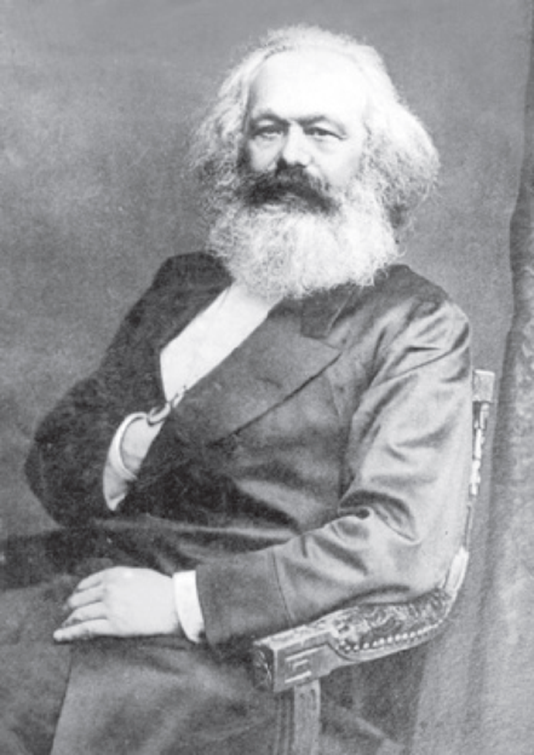
\includegraphics[width=\textwidth,height=0.99\textheight]{imgs3/img_slide57a.png}
\end{frame}

\begin{frame}{Which School of Thought Is Correct?}
\protect\hypertarget{which-school-of-thought-is-correct}{}
Which School of Thought Is Correct?

To date, we do not know which school of thought is correct about the
economy. + Many pieces of evidence can be interpreted in several
different ways. + Economists cannot isolate particular elements to study
and conduct controlled experiments.

So, it is likely that debate about the applicability of schools of
thought, and hence optimal policies for governments to pursue, will
continue for the foreseeable future.
\end{frame}

\begin{frame}{Copyright}
\protect\hypertarget{copyright}{}
Copyright

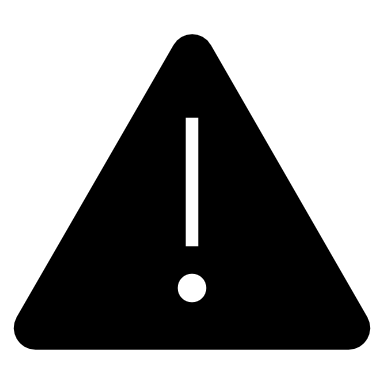
\includegraphics[width=\textwidth,height=0.99\textheight]{imgs3/img_slide59a.png}

This work is protected by United States copyright laws and is provided
solely for the use of instructors in teaching their courses and
assessing student learning. Dissemination or sale of any part of this
work (including on the World Wide Web) will destroy the integrity of the
work and is not permitted. The work and materials from it should never
be made available to students except by instructors using the
accompanying text in their classes. All recipients of this work are
expected to abide by these restrictions and to honor the intended
pedagogical purposes and the needs of other instructors who rely on
these materials.
\end{frame}

\end{document}
